\documentclass[11pt,a4paper]{article}

% --- PAQUETES PRINCIPALES ---
\usepackage[spanish,es-tabla]{babel} % Idioma español
\usepackage[margin=2.5cm]{geometry}
\usepackage{graphicx}
\usepackage{amsmath,amssymb,amsfonts}
\usepackage{booktabs}
\usepackage{csquotes}
\usepackage[backend=biber,style=ieee]{biblatex}
\addbibresource{referencias.bib}
\usepackage{hyperref}
\usepackage{caption}
\usepackage{subcaption}
\usepackage{float}
\usepackage{microtype}
\usepackage{enumitem}
\usepackage{tikz}
\usetikzlibrary{babel}

% Configuración de enlaces
\hypersetup{
    colorlinks=true,
    linkcolor=blue,
    filecolor=magenta,
    urlcolor=cyan,
    citecolor=blue,
    pdftitle={Documento Final - Proyecto Integrador II},
    pdfpagemode=FullScreen,
}

% --- DATOS DEL DOCUMENTO ---
\title{\textbf{\Large Maestría en Ciencia de Datos y Analítica (MCDA)}\\[0.3em]
\Large Proyecto Integrador II (2026-2)\\[1.5em]
\huge Predicción automática de tipos de roca a partir de registros de pozos petroleros}

\author{\textbf{Equipo 7}\\[0.5em]
Andrés Velasco \quad Daniel Pareja \quad Juan Morales \quad Santiago Molano \quad David Gómez}

\date{Noviembre 2026}

\begin{document}

\maketitle

\begin{abstract}
\noindent El presente documento constituye el informe técnico del proyecto integrador enfocado en la predicción automática de litofacies mediante series temporales multivariadas indexadas por profundidad a partir de registros geofísicos de pozos petroleros. Utilizando el conjunto de datos estandarizado FORCE 2020 (Mar del Norte), se abordan los desafíos de dependencia secuencial vertical, desbalance de clases extremo y generalización hacia pozos no vistos. Se integra un marco metodológico estructurado que abarca análisis estadístico avanzado de series temporales, arquitecturas de aprendizaje profundo (LSTM y Transformers) y principios de MLOps para un despliegue operativo en la nube.
\end{abstract}

\tableofcontents
\newpage

% ==========================================
% 1. INTRODUCCIÓN
% ==========================================
\section{Introducción}

\subsection{Contexto del problema}

Para conocer qué hay bajo la superficie, la industria de los hidrocarburos perfora pozos, agujeros de entre unos 15 y 66 centímetros de diámetro que pueden superar los cinco kilómetros de profundidad. El subsuelo que atraviesa un pozo está formado por capas de roca apiladas unas sobre otras, depositadas a lo largo de millones de años, y cada capa tiene su propio tipo de roca y su propio espesor. Saber qué roca hay a cada profundidad es la base de decisiones como dónde se encuentra un yacimiento, cómo construir su modelo y dónde perforar el siguiente pozo.

Para saber qué roca atraviesa un pozo existen dos vías. La más directa es recuperar cilindros de roca, llamados núcleos o testigos, pero hacerlo obliga a interrumpir la perforación y en un pozo en el mar eso resulta muy costoso, por lo que solo se toman en tramos cortos de especial interés. A lo largo de todo el pozo, la información principal proviene de herramientas que lo recorren midiendo de forma continua propiedades físicas de la roca, como su radiactividad natural, su densidad, la facilidad con que conduce la electricidad o la velocidad con que la atraviesa el sonido. Cada propiedad registrada a lo largo de la profundidad forma una curva, y el conjunto de curvas de un pozo se conoce como registro de pozo. En los datos de este proyecto hay una medición cada 0.152~m, unos 15~cm, de modo que un pozo reúne en promedio unas 12\,100 profundidades medidas (Figura~\ref{fig:contexto}).

Ninguna de estas curvas basta por sí sola para saber qué roca hay. Lo que permite reconocerla es su combinación, del mismo modo que un médico llega a un diagnóstico leyendo juntos varios exámenes y no uno solo. Con esa lectura, un geólogo asigna a cada profundidad un tipo de roca, como arenisca, lutita o caliza, y a ese tipo de roca interpretado lo llamamos en este documento litofacies. La decisión no se toma mirando cada medición aislada. Las capas tienen espesor, así que lo que aparece encima y debajo ayuda a distinguir si un cambio en las curvas marca el comienzo de una capa nueva o es solo una variación dentro de la misma.

Este trabajo de interpretación sigue siendo en buena parte manual. Es lento, porque cada pozo reúne miles de mediciones que se revisan tramo a tramo, y es subjetivo, porque dos especialistas pueden leer el mismo intervalo de manera distinta. Al mismo tiempo, la industria ha acumulado durante décadas los registros de un gran número de pozos. Automatizar una primera lectura, que el geólogo revise y corrija en lugar de construir desde cero, permitiría aprovechar ese volumen de información con mayor rapidez y con un mismo criterio para todos los pozos.

La Figura~\ref{fig:contexto} resume el planteamiento del proyecto. El modelo recibe las curvas de un pozo y entrega el tipo de roca a cada profundidad. Como las mediciones están ordenadas a lo largo del pozo, cada pozo se trata como una serie que avanza en profundidad, del mismo modo que una serie de tiempo avanza en el tiempo. La exigencia central es que el modelo funcione en pozos que nunca vio durante su entrenamiento, porque ese es el caso real de uso, un pozo nuevo que llega sin interpretar.

\begin{figure}[htbp]
\centering
\begin{tikzpicture}
\node[anchor=south west, inner sep=0] (img) at (0,0) {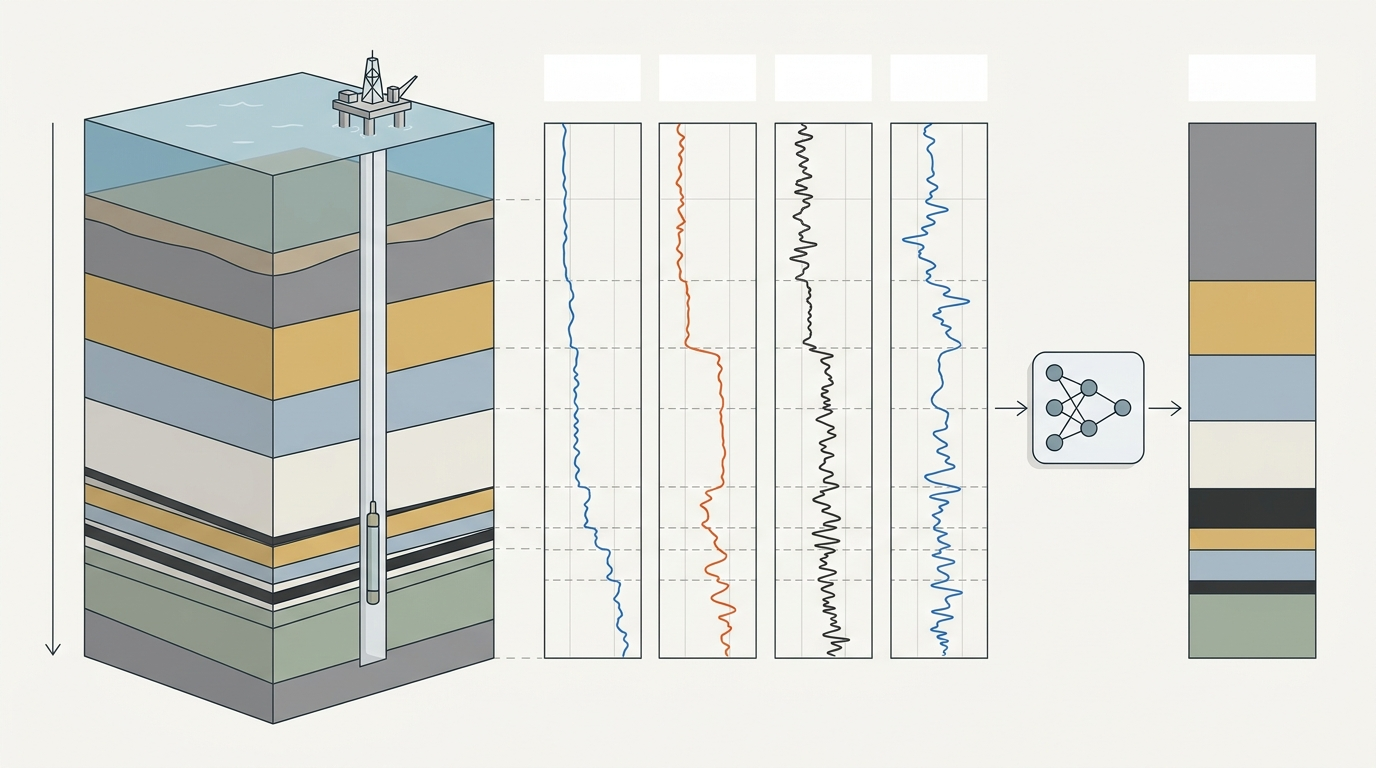
\includegraphics[width=\textwidth]{figuras/contexto_pozo.jpg}};
\begin{scope}[x={(img.south east)}, y={(img.north west)},
  lab/.style={font=\sffamily\fontsize{6}{7}\selectfont, text=black!80, align=center},
  tit/.style={font=\sffamily\bfseries\fontsize{7}{8.5}\selectfont, text=black!85, align=center}]
  \node[tit] at (0.200, 0.955) {Pozo que atraviesa capas de roca};
  \node[tit] at (0.556, 0.965) {Registros del pozo (una medición cada 15\,cm)};
  \node[lab] at (0.4300, 0.898) {Radiactividad};
  \node[lab] at (0.5144, 0.898) {Densidad};
  \node[lab] at (0.5985, 0.898) {Resistividad};
  \node[lab] at (0.6823, 0.898) {Sonido};
  \node[tit] at (0.7896, 0.355) {Modelo};
  \node[lab] at (0.9095, 0.898) {Tipo de roca\\predicho};
  \node[lab, rotate=90] at (0.020, 0.50) {Profundidad};
\end{scope}
\end{tikzpicture}
\caption{Esquema ilustrativo del problema. A la izquierda, un pozo perforado desde una plataforma en el mar atraviesa capas de roca de distinto tipo y espesor, y una herramienta que lo recorre mide propiedades físicas de la roca. En el centro, cada propiedad medida forma una curva a lo largo de la profundidad, y las curvas cambian de comportamiento justo en los límites entre capas (líneas punteadas). A la derecha, el modelo recibe las curvas y entrega el tipo de roca a cada profundidad. Las capas y las curvas son ilustrativas, no corresponden a datos reales y el dibujo no está a escala. Ilustración generada con IA y rotulada por el equipo.}
\label{fig:contexto}
\end{figure}

\subsection{Objetivo del proyecto}
El objetivo principal de este proyecto es implementar un sistema de aprendizaje automático secuencial y reproducible que prediga automáticamente la litofacies en cada profundidad de un pozo petrolero a partir de sus registros geofísicos. La solución busca servir como una herramienta de asistencia técnica que entregue una primera interpretación consistente para que el geólogo pueda revisar y ajustar, reduciendo los tiempos de procesamiento y evaluando su capacidad de generalizar a pozos completos nunca vistos por el modelo.

% ==========================================
% 2. MARCO TEÓRICO
% ==========================================
\section{Marco Teórico}

\subsection{Fundamentos de los métodos utilizados}
La predicción de litofacies se sitúa en la intersección entre la geofísica de subsuelo y el aprendizaje profundo aplicado a datos secuenciales:
\begin{itemize}
    \item \textbf{Registros de pozos y litofacies:} Un registro de pozo es una serie multivariada indexada por profundidad. Una litofacies define una unidad de roca con propiedades físicas y composicionales homogéneas.
    \item \textbf{Dependencia secuencial y contexto vertical:} A diferencia de los datos tabulares independientes, las capas de roca presentan continuidad física, ciclos sedimentarios y gradaciones. Por ende, la respuesta geofísica en una profundidad $d$ depende fuertemente del contexto vertical adyacente ($d \pm k$).
    \item \textbf{Redes Neuronales Secuenciales y Atención:} Para capturar dependencias a corto y largo alcance, se recurre a arquitecturas de Redes Neuronales Recurrentes con memoria (LSTM) y modelos basados en mecanismos de atención (Transformers), capaces de aprender representaciones jerárquicas del contexto vertical.
    \item \textbf{Validación cruzada por grupos (Group K-Fold):} Debido a la alta autocorrelación espacial/vertical dentro de un mismo pozo, las particiones de datos tradicionales introducen fuga de información (\emph{data leakage}). La evaluación debe realizarse aislando pozos completos en los conjuntos de validación y prueba.
\end{itemize}

\subsection{Referencias}
El desarrollo teórico y metodológico se fundamenta en la literatura especializada reciente sobre aprendizaje profundo aplicado a geociencias \cite{xie2024, carvalho2026, bormann2020, jamshidi2023, zhao2025}.

% ==========================================
% 3. DESARROLLO METODOLÓGICO
% ==========================================
\section{Desarrollo Metodológico}

\subsection{Problema}

\subsubsection{Definición del problema}
\label{sec:definicion-problema}

Desde el punto de vista del negocio, el problema es producir de forma automática una primera interpretación del tipo de roca a lo largo de un pozo a partir de sus registros, consistente entre pozos, que el geólogo pueda revisar en lugar de elaborar desde cero. Su valor depende de una condición que guía todo el proyecto. El sistema debe funcionar sobre pozos que no formaron parte de su entrenamiento, porque en la práctica cada pozo que llega para ser interpretado es un pozo nuevo.

Desde el punto de vista técnico, se trata de un problema de clasificación supervisada. Es de clasificación porque la respuesta es una categoría, una de 12 clases de roca, y no un número, y es supervisada porque el modelo aprende de ejemplos cuya respuesta correcta ya se conoce, en este caso la litofacies que interpretaron geólogos en 118 pozos del Mar del Norte. Lo que lo distingue de una clasificación corriente es que los ejemplos no son independientes entre sí. Las mediciones de un pozo forman una secuencia ordenada por profundidad, y la notación de las series de tiempo describe bien esa estructura si el índice $t$ se interpreta como la posición a lo largo del pozo en lugar de un instante de tiempo.

Para un pozo $w$ con $n_w$ profundidades medidas y $p$ curvas, las mediciones forman la serie multivariada
\begin{equation}
\mathbf{x}_{w,t} = \left(x_{w,t}^{(1)}, \dots, x_{w,t}^{(p)}\right)^{\top}, \qquad t = 1, \dots, n_w ,
\end{equation}
donde $x_{w,t}^{(j)}$ es el valor de la curva $j$ en la posición $t$ del pozo $w$, y dos posiciones consecutivas están separadas por 0.152~m. A cada posición le corresponde una etiqueta $y_{w,t} \in \{1, \dots, 12\}$, que es la litofacies interpretada. Un modelo punto a punto predice la etiqueta de cada profundidad usando solo las mediciones de esa misma profundidad, $\hat{y}_{w,t} = f(\mathbf{x}_{w,t})$. Un modelo con contexto vertical usa además las $h$ posiciones de arriba y las $h$ de abajo,
\begin{equation}
\hat{y}_{w,t} = f\left(\mathbf{x}_{w,t-h}, \dots, \mathbf{x}_{w,t}, \dots, \mathbf{x}_{w,t+h}\right),
\end{equation}
de modo que observa una ventana de $W = 2h + 1$ posiciones centrada en la profundidad que se quiere clasificar. El tamaño de esa ventana no se elige por ensayo y error, sino que se deriva con evidencia estadística en el análisis exploratorio de este documento.
% Pendiente: agregar \ref a la subsección donde se deriva W cuando exista su etiqueta.

Los modelos se ajustan con un conjunto de pozos de entrenamiento $\mathcal{W}_{\text{ent}}$ y se evalúan sobre un conjunto de pozos de prueba $\mathcal{W}_{\text{prueba}}$ que no comparte ningún pozo con el primero, $\mathcal{W}_{\text{ent}} \cap \mathcal{W}_{\text{prueba}} = \varnothing$. Ningún pozo aporta filas a más de un conjunto.

Desde el punto de vista científico, la pregunta es cuánto mejora la predicción al incorporar el contexto vertical y si esa mejora se mantiene en pozos no vistos. Responderla exige comparar, bajo un mismo protocolo de evaluación, modelos que no usan contexto con modelos que sí lo usan.

El problema presenta cuatro dificultades que condicionan las decisiones del proyecto.

La primera es la fuerte dependencia entre profundidades vecinas. En la curva GR, que mide la radiactividad natural de la roca, la correlación entre cada medición y la siguiente, 0.152~m más abajo, es de 0.991 en el conjunto de pozos (a esta correlación de una serie consigo misma desplazada se le llama autocorrelación). Si las filas de un mismo pozo se repartieran al azar entre entrenamiento y prueba, casi cada fila de prueba tendría una vecina prácticamente idéntica en el entrenamiento, y el modelo obtendría un resultado alto sin haber aprendido a generalizar. Este fenómeno se conoce como fuga de información y es la razón por la que la partición se hace siempre por pozo completo.

La segunda es el desbalance de clases. La lutita (\emph{Shale}, roca de grano muy fino formada por arcilla compactada) ocupa el 61.3\,\% de las profundidades etiquetadas, y junto con la arenisca (\emph{Sandstone}, arena compactada y cementada) y la intercalación fina de ambas (\emph{Sandstone/Shale}) suma el 88.4\,\%. Un modelo que respondiera siempre lutita acertaría seis de cada diez veces sin haber aprendido nada, por lo que el porcentaje global de aciertos no basta para medir el desempeño. Además, las clases raras se concentran en muy pocos pozos. El basamento (\emph{Basement}, roca cristalina antigua situada debajo de las capas sedimentarias) aparece en un único pozo, la sal (\emph{Halite}) en 4, la anhidrita (\emph{Anhydrite}, sulfato de calcio emparentado con el yeso) en 10 y la creta (\emph{Chalk}, carbonato muy fino y blando) en 15. Como cada pozo pertenece a un solo conjunto, no todas las clases pueden estar presentes a la vez en entrenamiento, validación y prueba.

La tercera es la heterogeneidad de las mediciones. El conjunto de datos incluye 20 curvas, pero no todas se midieron en todos los pozos, porque cada operador decide qué herramientas usar según el costo y el propósito del pozo. Solo cinco curvas están presentes en los 118 pozos, ningún pozo tiene las 20 (el más completo tiene 18) y a cada pozo le faltan en promedio casi siete curvas que nunca se registraron. A esto se suman tramos sin dato dentro de curvas que sí se midieron y saltos de profundidad sin ningún registro. El modelo debe trabajar, por lo tanto, con entradas incompletas y que cambian de un pozo a otro.

La cuarta es que la etiqueta es una interpretación y no una medición directa. La litofacies de referencia la asignaron geólogos, con el grado de subjetividad descrito en la introducción, y en 108 de los 118 pozos el conjunto de datos registra la confianza del intérprete en una escala de 1 a 3. El modelo aprende a reproducir esa interpretación, con sus posibles inconsistencias.

\subsubsection{Hipótesis}

Las hipótesis se plantean como comparaciones entre modelos evaluados sobre pozos completos que no se usaron en el entrenamiento, con las mismas particiones y las mismas métricas para todos.

\begin{enumerate}[label=\textbf{H\arabic*.}, leftmargin=*]
    \item Incorporar el contexto vertical, es decir, las mediciones de las profundidades vecinas, mejora la predicción del tipo de roca frente a un modelo que clasifica cada profundidad solo con sus propias mediciones.
    \item Los modelos de aprendizaje profundo aprovechan ese contexto mejor que los modelos estadísticos de referencia, porque además de la continuidad de las capas pueden reconocer la forma de las curvas a lo largo del pozo.
\end{enumerate}

\subsection{Datos}

\subsubsection{Fuentes de datos}

El proyecto utiliza el conjunto de datos abierto FORCE 2020 \cite{bormann2020}, publicado para una competencia de aprendizaje automático realizada en Noruega en 2020, cuyo reto era precisamente predecir el tipo de roca a partir de registros de pozo. Reúne los registros de 118 pozos perforados en el Mar del Norte, frente a la costa noruega, junto con la litofacies que interpretaron geólogos en cada profundidad. Los registros originales provienen de la autoridad petrolera de Noruega (Sodir, antes NPD), que los publica como datos abiertos.

El uso de los datos en el proyecto está permitido por sus licencias. El conjunto compilado se distribuye con licencia Creative Commons Atribución 4.0 (CC BY 4.0), que permite usarlo libremente siempre que se cite a sus autores, y los registros originales están cubiertos por la Licencia Noruega de Datos Abiertos (NOLD 2.0).

La referencia oficial del conjunto es su registro en Zenodo, con identificador DOI, y la copia de trabajo es el repositorio público de la competencia en GitHub \cite{force2020repo}, donde los datos están en archivos de texto con columnas separadas por punto y coma. El cuaderno de trabajo lee los archivos directamente desde ese repositorio cada vez que se ejecuta, sin copias manuales intermedias, para que cualquier miembro del equipo parta exactamente de los mismos datos. Antes de usarlos, se verificó su integridad comparando el tamaño en bytes y la huella digital (\emph{hash}) de cada archivo con los que reporta el propio repositorio. Una huella digital es un código calculado a partir del contenido de un archivo, que cambia por completo si se altera un solo carácter. Los cinco archivos utilizados coincidieron. El mismo repositorio conserva además los archivos originales de 71 pozos en formato LAS, el formato estándar de la industria para registros de pozo, que se consultaron solo para confirmar unidades de medida y el paso de muestreo.

La competencia repartió los pozos en tres grupos, resumidos en la Tabla~\ref{tab:grupos}. En el grupo de la tabla de posiciones, las mediciones y las etiquetas venían en dos archivos separados, que se unieron por nombre de pozo y profundidad sin que quedaran filas sueltas ni duplicadas.

\begin{table}[htbp]
\centering
\caption{Grupos de pozos definidos por la competencia FORCE 2020.}
\label{tab:grupos}
\begin{tabular}{llrr}
\toprule
\textbf{Grupo} & \textbf{Papel en la competencia} & \textbf{Pozos} & \textbf{Filas} \\
\midrule
\texttt{train} & entrenamiento, con etiqueta & 98 & 1\,170\,511 \\
\texttt{hidden\_test} & prueba ciega & 10 & 122\,397 \\
\texttt{leaderboard\_test} & prueba para la tabla de posiciones & 10 & 136\,786 \\
\midrule
Total & & 118 & 1\,429\,694 \\
\bottomrule
\end{tabular}
\end{table}

Durante la competencia, las etiquetas de los dos grupos de prueba eran secretas, pero se publicaron al cerrarla, y desde entonces circulan soluciones ajustadas a esos pozos. Por eso ya no pueden funcionar como una prueba ciega. En lugar de descartarlos, los 118 pozos se reunieron en un único conjunto y el equipo define su propia partición en entrenamiento, validación y prueba, siempre por pozo completo. Una vez hecho ese reparto, el grupo de origen de cada pozo en la competencia deja de tener relevancia. Como precaución adicional, el equipo evita consultar soluciones publicadas de la competencia para los pozos que terminen en el conjunto de prueba propio.
% Pendiente Etapa 4: \ref a la subsección del protocolo de evaluación.

\subsubsection{Descripción y naturaleza}

Los datos son estructurados, es decir, están organizados en una tabla con columnas fijas, y llegan como un único lote histórico de archivos y no como un flujo continuo de mediciones. Al reunir los tres grupos de la competencia se obtiene una tabla de 1\,429\,694 filas y 30 columnas, de unos 157~MB. Cada fila corresponde a una profundidad dentro de un pozo y contiene todas las mediciones tomadas en ella. La profundidad es la profundidad medida (MD, por sus siglas en inglés), es decir, la distancia recorrida a lo largo del pozo desde la superficie, y avanza de una fila a la siguiente en pasos de 0.152~m. Un pozo tiene en promedio unas 12\,100 filas, con extremos entre 1\,734 y 25\,131.

Aunque la tabla es una sola, contiene 118 series apiladas una debajo de otra. Para reconstruir la serie de un pozo basta agrupar por su nombre y ordenar por profundidad. Dos filas consecutivas de la tabla pueden pertenecer a pozos distintos, por lo que cualquier cálculo que dependa del orden se hace siempre dentro de cada pozo. Dentro de un mismo pozo la profundidad siempre aumenta, pero no siempre de forma continua. En 61 pozos el registro no tiene interrupciones, mientras que los otros 57 presentan entre 1 y 11 saltos, tramos en los que no se registró ninguna medición, el mayor de ellos de 269~m. Al cortar cada pozo en esos saltos se obtienen 296 tramos continuos, que son la verdadera unidad sobre la que se analizan las series.

Las 30 columnas se agrupan en cinco tipos. Cinco identifican el pozo y la posición de cada fila (\texttt{WELL}, \texttt{DEPTH\_MD} y las coordenadas \texttt{X\_LOC}, \texttt{Y\_LOC} y \texttt{Z\_LOC}). Dos son categóricas y dan el nombre oficial de la unidad de roca en la nomenclatura noruega, \texttt{GROUP} con 14 categorías y \texttt{FORMATION} con 70, que es una subdivisión de la anterior. Veinte son las curvas de registro, que constituyen las entradas de los modelos (Tabla~\ref{tab:curvas}). Dos corresponden a la etiqueta, la litofacies codificada como número (\texttt{FORCE\_2020\_LITHOFACIES\_LITHOLOGY}) y la confianza del intérprete en una escala de 1 a 3 (\texttt{FORCE\_2020\_LITHOFACIES\_CONFIDENCE}). La última, \texttt{source}, la agregó el equipo para registrar el grupo de origen en la competencia.

El conjunto de datos no incluye un diccionario oficial con las unidades de cada curva. Se buscó en el registro de Zenodo, en el repositorio de la competencia y en su informe técnico, sin éxito. Por eso cada unidad se estableció combinando la convención estándar de la industria con la comprobación de que los valores observados en los 118 pozos son físicamente razonables bajo esa unidad. Por ejemplo, se verificó que la porosidad neutrón viene como fracción entre 0 y 1 y no como porcentaje.

\begin{table}[htbp]
\centering
\small
\caption{Curvas de registro del conjunto de datos, agrupadas según lo que describen.}
\label{tab:curvas}
\begin{tabular}{lp{8.2cm}l}
\toprule
\textbf{Curva} & \textbf{Qué mide} & \textbf{Unidad} \\
\midrule
\multicolumn{3}{l}{\emph{Propiedades de la roca}} \\
\texttt{GR} & Radiactividad natural (rayos gamma), mayor en arcillas que en arenas limpias & API \\
\texttt{SGR} & Variante espectral de los rayos gamma & API \\
\texttt{RHOB} & Densidad de la roca & g/cm$^3$ \\
\texttt{NPHI} & Porosidad neutrón, ligada a la cantidad de fluido en los poros & fracción \\
\texttt{PEF} & Factor fotoeléctrico, ligado a la composición mineral & barns/electrón \\
\texttt{DTC} & Tiempo que tarda una onda de compresión en recorrer un pie de roca & $\mu$s/pie \\
\texttt{DTS} & Lo mismo que \texttt{DTC} para una onda de corte & $\mu$s/pie \\
\texttt{RDEP}, \texttt{RMED}, \texttt{RSHA} & Resistividad eléctrica a distancia profunda, media y somera de la pared del pozo & ohm$\cdot$m \\
\texttt{RMIC}, \texttt{RXO} & Resistividad muy cerca de la pared, en la zona invadida por el lodo & ohm$\cdot$m \\
\texttt{SP} & Potencial espontáneo, un voltaje natural entre el lodo y la roca & mV \\
\midrule
\multicolumn{3}{l}{\emph{Estado del pozo y operación de perforación}} \\
\texttt{CALI} & Diámetro real del agujero & pulgadas \\
\texttt{BS} & Diámetro de la broca con que se perforó & pulgadas \\
\texttt{DCAL} & Diferencia entre el diámetro real y el de la broca & pulgadas \\
\texttt{DRHO} & Corrección aplicada a la densidad por mal contacto con la pared & g/cm$^3$ \\
\texttt{ROP}, \texttt{ROPA} & Velocidad de avance de la broca y su promedio & m/h (probable) \\
\texttt{MUDWEIGHT} & Densidad del lodo de perforación & g/cm$^3$ \\
\bottomrule
\end{tabular}
\end{table}

No todas las curvas se midieron en todos los pozos (Figura~\ref{fig:curvas}). Solo cinco (\texttt{GR}, \texttt{RDEP}, \texttt{NPHI}, \texttt{DTC} y \texttt{RHOB}) están presentes en los 118, y otras, como \texttt{SGR}, \texttt{DCAL} o \texttt{MUDWEIGHT}, aparecen en menos de un tercio de ellos. El patrón es coherente con la práctica de la industria, en la que un paquete básico de herramientas se corre en casi todos los pozos y las más costosas o especializadas solo en algunos.

\begin{figure}[htbp]
\centering
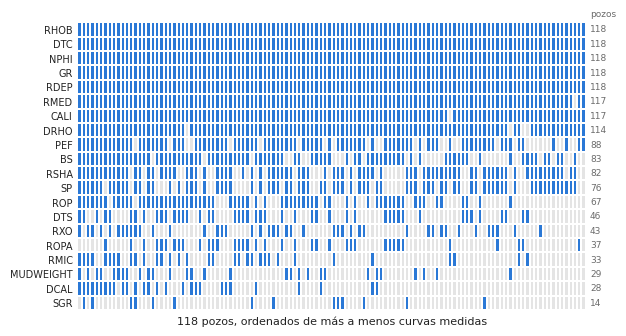
\includegraphics[width=\textwidth]{figuras/informe_curvas_por_pozo.png}
\caption{Curvas medidas en cada pozo. Cada columna es un pozo y cada fila una curva. En azul aparecen las curvas que se midieron en ese pozo y en gris las que nunca se midieron, y a la derecha el número de pozos que tienen cada curva. Los pozos están ordenados de más a menos curvas medidas. Datos de la Etapa 1, antes de la curación.}
\label{fig:curvas}
\end{figure}

La etiqueta distingue 12 tipos de roca. La correspondencia entre cada código numérico y su nombre se verificó contra el cuaderno oficial del repositorio de la competencia y cubre todos los códigos presentes. La Tabla~\ref{tab:clases} los describe junto con su frecuencia y el número de pozos en que aparecen.

\begin{table}[htbp]
\centering
\small
\caption{Tipos de roca de la etiqueta, porcentaje de las profundidades etiquetadas y número de pozos en que aparecen.}
\label{tab:clases}
\begin{tabular}{lp{6.6cm}rr}
\toprule
\textbf{Clase} & \textbf{Descripción} & \textbf{\%} & \textbf{Pozos} \\
\midrule
\emph{Shale} (lutita) & Arcilla y lodo compactados, de grano muy fino & 61.31 & 118 \\
\emph{Sandstone} (arenisca) & Arena compactada y cementada & 14.48 & 118 \\
\emph{Sandstone/Shale} & Intercalación fina de arenisca y lutita & 12.61 & 117 \\
\emph{Limestone} (caliza) & Carbonato de calcio, a menudo de origen marino & 4.86 & 114 \\
\emph{Marl} (marga) & Mezcla de arcilla y carbonato & 2.87 & 92 \\
\emph{Tuff} (toba) & Ceniza volcánica compactada & 1.22 & 67 \\
\emph{Halite} (sal) & Sal de roca & 1.03 & 4 \\
\emph{Chalk} (creta) & Carbonato muy fino y blando, como la tiza & 0.98 & 15 \\
\emph{Coal} (carbón) & Restos vegetales compactados & 0.33 & 63 \\
\emph{Dolomite} (dolomía) & Carbonato de calcio y magnesio & 0.17 & 47 \\
\emph{Anhydrite} (anhidrita) & Sulfato de calcio, emparentado con el yeso & 0.13 & 10 \\
\emph{Basement} (basamento) & Roca cristalina antigua bajo las capas sedimentarias & 0.01 & 1 \\
\bottomrule
\end{tabular}
\end{table}

\subsection{Análisis Exploratorio de Datos (EDA)}
\label{sec:eda}

El análisis exploratorio tiene aquí dos propósitos. El primero es conocer los datos lo suficiente para confiar en ellos y prepararlos sin introducir información inventada. El segundo es caracterizar cómo se comportan las curvas a lo largo del pozo, para que las decisiones de diseño del modelo, en particular cuánto contexto vertical debe observar, se apoyen en evidencia estadística y no en ensayo y error. El recorrido sigue ese orden. Primero se revisa la calidad de los datos tal como vienen (sección~\ref{sec:eda-entendimiento}), luego se describen las reglas con que se corrigieron (sección~\ref{sec:eda-limpieza}), después se analiza cada curva como serie a lo largo de la profundidad (sección~\ref{sec:eda-descriptivo}) y por último se estudian las relaciones entre curvas y los cambios de roca, de donde se deriva el tamaño de la ventana de contexto (sección~\ref{sec:eda-patrones}).

Todo el análisis respeta una regla que protege la validez de la evaluación posterior. Un paso puede hacerse sobre los 118 pozos solo si no usa la litofacies y no depende de qué pozos terminen en el conjunto de prueba. Cumplen esta condición el examen de las curvas, la aplicación de límites físicos, que son constantes de la naturaleza, y los cálculos que usan únicamente los datos de un pozo y se aplican a ese mismo pozo. En cambio, los cálculos que combinan información de varios pozos, como una media global para escalar una curva, se aplazan hasta después de la partición y se harán solo con los pozos de entrenamiento. Del mismo modo, ningún análisis de esta sección usa la litofacies. Las comparaciones que la requieren, como contrastar los cambios detectados en las curvas con los cambios de roca interpretados, quedan para la etapa de modelado y se harán también solo con pozos de entrenamiento. Las columnas \texttt{GROUP} y \texttt{FORMATION}, que nombran las unidades de roca pero no son la variable que se quiere predecir, sí se usan como referencia externa.

\subsubsection{Entendimiento de los datos}
\label{sec:eda-entendimiento}

Antes de analizar las curvas se revisó qué tan confiables son los datos tal como vienen. La primera comprobación fue la cobertura de la etiqueta. No bastaba con que cada pozo tuviera la columna de litofacies, porque un pozo puede tenerla y aun así dejar tramos sin interpretar. Por eso se contó, pozo por pozo, cuántas filas tienen una etiqueta válida. Los 118 pozos están etiquetados en el 100\,\% de sus filas, y no hay nombres de pozo repetidos entre los tres grupos de la competencia, de modo que se trata de 118 pozos distintos.

La segunda comprobación se refiere a los valores faltantes. Cuando a una curva le faltan datos en un pozo pueden estar ocurriendo dos cosas muy diferentes. Puede que la herramienta nunca se haya usado en ese pozo, y entonces falta la curva completa, o puede que sí se haya usado y falten lecturas en algunos tramos, por ejemplo donde el pozo estaba revestido o donde el agujero se derrumbó. Distinguirlas importa porque no tiene sentido intentar recuperar una curva que nunca existió. De las 2\,360 combinaciones posibles de pozo y curva, 676 están completas, 796 corresponden a curvas que nunca se midieron y 888 tienen faltantes parciales. La separación entre los dos primeros casos no requirió elegir un umbral, porque los datos la muestran de forma limpia. Ninguna curva tiene un faltante cercano pero inferior al 100\,\%, así que una curva no medida se define simplemente como la que falta por completo. Entre los faltantes parciales se observó además un patrón con explicación física. En 135 casos falta un único tramo pegado a un extremo del pozo, casi siempre el superior (117 de los 135), y se concentra en herramientas que necesitan contacto con la pared del agujero. Es lo esperable cuando esa parte del pozo está recubierta con tubería de acero, a través de la cual esas herramientas no pueden medir.

La tercera comprobación buscó valores que parecen mediciones pero no lo son. En cuatro curvas, la ausencia de dato no aparece como una celda vacía sino como un número convencional, llamado centinela, del tipo $-999$ (Tabla~\ref{tab:centinelas}). En tres de ellas su peso es despreciable, pero en la resistividad de la zona lavada (\texttt{RXO}) casi una de cada diez lecturas aparentemente válidas era en realidad un centinela. Tomado como dato, un valor de $-999$ en una resistividad, que físicamente no puede ser negativa, distorsionaría cualquier promedio y cualquier modelo. Al convertir estos valores en faltantes apareció un problema adicional. Los computadores guardan los números decimales con una precisión limitada, y parte de los $-999.9$ estaba almacenada como $-999.900024$, por lo que una comparación exacta no los reconocía. Comparar con una tolerancia de 0.01 resolvió el problema y elevó el faltante total de \texttt{RXO} de 75.66\,\% a 76.80\,\%.

\begin{table}[htbp]
\centering
\small
\caption{Valores centinela encontrados en las curvas, es decir, números que representan la ausencia de dato.}
\label{tab:centinelas}
\begin{tabular}{llrr}
\toprule
\textbf{Curva} & \textbf{Valor centinela} & \textbf{Casos} & \textbf{\% de las lecturas no vacías} \\
\midrule
\texttt{SP}   & $-999.0$            & 402      & 0.04 \\
\texttt{RMIC} & $10\,000.0$         & 3        & $<0.01$ \\
\texttt{ROPA} & $-999.25$           & 24       & 0.01 \\
\texttt{RXO}  & $-999.0$ y $-999.9$ & 34\,481  & 9.41 \\
\bottomrule
\end{tabular}
\end{table}

La revisión encontró también valores aislados físicamente imposibles que no siguen el patrón de un centinela, como un diámetro de agujero de más de 10\,000 pulgadas, una corrección de densidad de $-7\,429$~g/cm$^3$ o una velocidad de perforación de 47\,015~m/h. Su tratamiento se describe en la sección~\ref{sec:eda-limpieza}. Por último, las tres coordenadas de ubicación faltan juntas en el 0.76\,\% de las filas, lo que apunta a un problema de posicionamiento en tramos puntuales y no a errores independientes en cada coordenada.

Esta revisión dejó una lección de método que se aplicó en todo el proyecto. Un dato no se considera verificado porque se vea bien en pantalla, sino cuando se comprueba contra la fuente y con la precisión real. El paso entre mediciones, por ejemplo, se había registrado al principio como 0.1524~m (medio pie), porque en pantalla, con tres decimales, ese valor y 0.152 se ven idénticos. La cabecera del archivo original y los valores de profundidad confirmaron que el paso real es 0.152~m.

\subsubsection{Preparación y limpieza}
\label{sec:eda-limpieza}

La limpieza se rigió por un principio general. Es preferible dejar un hueco reconocible que introducir un número inventado, porque un valor inventado se ve igual que uno medido y el modelo no tiene forma de distinguirlos. Con esa preferencia, cada dato problemático recibió uno de cuatro tratamientos. Por defecto se enmascaró, es decir, se convirtió en faltante. Se corrigió solo cuando existía un patrón sistemático, reproducible y verificado que permitiera recuperar el valor correcto. Se marcó con una bandera, sin modificarlo, cuando el valor era extraño pero contenía información física real. Y se imputó, es decir, se rellenó con un valor estimado, solo cuando había datos reales a ambos lados y a una distancia justificada. Todas las reglas quedaron escritas como funciones en el cuaderno de trabajo, de modo que se aplican de nuevo desde cero y producen siempre el mismo resultado, y cada una se verificó comprobando que los conteos antes y después cuadraran exactamente.

\paragraph{Valores faltantes.} La unidad de decisión no fue la curva completa en un pozo, sino cada tramo faltante por separado, porque una misma curva puede tener faltantes de naturaleza distinta. La regla distingue dos casos según dónde esté el tramo. Un tramo faltante que toca el borde de un tramo continuo de registro, ya sea el inicio o el final del pozo o uno de sus saltos de profundidad, nunca se rellena. Estimarlo sería extrapolar, es decir, inventar valores con información de un solo lado, y no hay forma de comprobar el resultado. Esta sola regla resuelve las curvas que nunca se midieron, cuyo pozo completo es borde, los tramos faltantes en la parte superior del pozo y la mayoría de los casos de faltantes extensos. Los tramos interiores, que tienen datos reales arriba y abajo, sí admiten interpolación, pero solo hasta una distancia máxima. Por encima de ella, el hueco podría ocultar una capa de roca distinta que la interpolación borraría. Esa distancia, de 8 posiciones (1.2~m), no se fijó a ojo sino a partir de la resolución propia de las curvas (sección~\ref{sec:eda-patrones}).

Los huecos interiores son una fracción pequeña del problema. Suman 193\,674 celdas, repartidas en 2\,226 huecos, y aunque el 61\,\% de esos huecos mide 8 posiciones o menos, en conjunto solo representan 4\,818 celdas, el 2.5\,\% de las celdas interiores. El 86\,\% de ellas está en huecos de más de 100 posiciones (más de 15~m), que corresponden a intervalos donde la curva no se registró y que quedan como faltantes. La interpolación de los huecos cortos no se aplicó sobre el conjunto curado. Se aplicará en la preparación de los datos para el modelo, de forma lineal, usando solo los dos vecinos del mismo tramo y agregando una columna que marca qué valores fueron interpolados, para que el modelo pueda distinguirlos.
% Pendiente: \ref a la subsección del pipeline de datos (3.4 o 4.2) cuando exista.
\paragraph{Valores fuera de rango físico.} Para decidir qué valores son imposibles se usaron límites físicos de la industria y no el rango observado en los datos. Usar el rango observado sería circular, porque se calcula con los mismos datos que se quieren revisar, errores incluidos, y un valor erróneo extremo quedaría validado por definición. Un límite físico, en cambio, es una constante de la naturaleza. Los rayos gamma no pueden ser negativos, la porosidad no puede superar el 100\,\% y la densidad de una roca está entre 1.0 y 3.6~g/cm$^3$. Además, como no depende de ningún pozo, aplicarlo a los 118 no genera fuga de información. Los valores fuera de esos límites se enmascararon.

\paragraph{Correcciones y exclusiones.} Solo una curva cumplió las condiciones para ser corregida. En el peso del lodo de perforación (\texttt{MUDWEIGHT}), cuya unidad no figura en ninguna fuente, la mediana de cada uno de los 29 pozos que la tienen cae en uno de tres niveles separados exactamente por potencias de diez. Al reescalar cada pozo con el orden de magnitud de su propia mediana, las 29 medianas quedan entre 1.08 y 1.80~g/cm$^3$, el rango esperado para un lodo de perforación. El patrón es sistemático y verificable, y la corrección de cada pozo usa solo sus propios datos. Cuando no existió un patrón así, la curva no confiable se excluyó completa en el pozo afectado en lugar de corregirla. Es el caso de la corrección de densidad (\texttt{DRHO}) en dos pozos donde la columna resultó ser una copia o una mezcla de la densidad misma, y de la velocidad de perforación (\texttt{ROP}) en un pozo cuya mediana, de 17\,778~m/h, es imposible en cualquier unidad.

\paragraph{Bandera en lugar de borrado.} El factor fotoeléctrico (\texttt{PEF}) presenta muchos valores por encima de 10, que ningún mineral común alcanza. La explicación más probable es la barita que se agrega al lodo para hacerlo más pesado, cuyo factor fotoeléctrico ronda 267. Esos valores no son un error del instrumento, sino información real sobre las condiciones del pozo, así que no se borraron. Se conservaron y se agregó una columna que marca las 75\,106 filas afectadas, cerca del 8.5\,\% de las lecturas de esa curva. Cómo usar esa marca en el modelo se decidirá en la etapa de modelado.

\paragraph{Lecturas que no miden la roca.} La revisión detallada encontró tramos en los que el instrumento registraba algo distinto de la roca. En tres pozos se identificó con el diámetro del agujero el tramo superior aún revestido con tubería, donde varias herramientas no pueden medir, y se enmascararon todas las curvas por encima de ese punto. También se enmascararon arranques de instrumento, como lecturas fijas en el mínimo detectable justo después de un salto de profundidad, y canales congelados. Para estos últimos se adoptó una regla general. Como cada lectura resume aproximadamente el metro de roca que la rodea, una curva de formación no puede repetir exactamente el mismo valor durante 20 lecturas seguidas (3~m), y toda racha así se enmascaró. La regla afectó 13\,869 celdas en 14 curvas, entre ellas una racha de 3\,759 ceros en la corrección de densidad de un pozo y un canal de potencial espontáneo muerto en todo un pozo.

\paragraph{Potencial espontáneo.} El potencial espontáneo (\texttt{SP}) recibió un tratamiento propio porque es una medición relativa. No tiene un cero absoluto y su nivel de referencia puede desplazarse entre corridas de la herramienta sin que cambie la roca. En cuatro pozos se encontró un salto de nivel de este tipo, que se corrigió restando la diferencia entre las medianas de antes y después del salto, sin alterar la forma de la señal. Se distinguieron además estos saltos reales de picos aislados en los empalmes de corridas, que no implican un cambio de nivel, y se enmascararon algunos tramos degenerados. Tres anomalías sin causa confirmada quedaron documentadas sin tratamiento, porque corregirlas sin evidencia sería inventar.

\paragraph{Paso de muestreo.} Todos los pozos comparten exactamente el mismo paso de 0.152~m, y los 178 saltos de profundidad son múltiplos enteros de ese paso, de modo que en ningún pozo cambió la frecuencia de medición. Por eso no fue necesario remuestrear los datos a una malla común, lo que habría obligado a calcular valores en profundidades donde no se midió. Los saltos tampoco se rellenaron. A diferencia de un hueco en una sola curva, donde las demás curvas sí tienen dato, en un salto de profundidad no existe ninguna medición. Cada salto se trata como un límite tan firme como el final de un pozo, y cada pozo queda dividido en tramos continuos, 296 en total, que serán la unidad sobre la que se construyan las ventanas de contexto del modelo.

\paragraph{Normalización.} Las curvas tienen escalas muy distintas. Los rayos gamma alcanzan cientos de unidades, la densidad ronda 2.4~g/cm$^3$ y la resistividad varía entre décimas y miles de ohm$\cdot$m. Muchos modelos, y en particular las redes neuronales, aprenden mal cuando sus entradas tienen escalas tan diferentes, porque las variables de valores grandes dominan el aprendizaje. Normalizar consiste en llevar todas las curvas a una escala comparable, y para cada una se tomaron tres decisiones en orden.

La primera fue si transformarla con un logaritmo. Se aplicó el logaritmo en base 10 solo a las curvas en las que importa cuántas veces cambia el valor y no cuánto, como ocurre con la resistividad, donde pasar de 1 a 10~ohm$\cdot$m equivale físicamente a pasar de 100 a 1\,000. Se transformaron así las cinco resistividades, el factor fotoeléctrico y las dos velocidades de perforación.

La segunda fue si la escala debía calcularse con todos los pozos a la vez, de forma global, o con cada pozo por separado. Algunas curvas cambian de nivel de un pozo a otro por razones ajenas a la roca, como la calibración de la herramienta o el tipo de lodo. Si se normalizan de forma global, el modelo puede aprender a reconocer el pozo por su nivel típico en lugar de reconocer la roca, un atajo que funciona en entrenamiento y falla en un pozo nuevo. Para decidir se usó el cociente
\begin{equation}
r = \frac{s_{\text{entre}}}{\mathrm{IQR}_{\text{dentro}}} ,
\end{equation}
donde $s_{\text{entre}}$ es la desviación estándar de las medianas de la curva en los distintos pozos, y mide cuánto cambia su nivel típico de un pozo a otro, e $\mathrm{IQR}_{\text{dentro}}$ es la mediana, entre pozos, del rango intercuartílico de cada pozo, es decir, del ancho del 50\,\% central de sus valores, y mide cuánto varía la curva dentro de un mismo pozo por el paso de una capa a otra. Si $r \geq 1$, el salto de nivel entre pozos es al menos tan grande como la variación geológica interna, y la curva se normaliza por pozo. Si $r < 1$, se normaliza de forma global. El umbral es un criterio propio del equipo y se aplicó sin excepciones, incluso en casos cercanos a él. Con esta regla, seis curvas se normalizan por pozo (\texttt{SP}, \texttt{SGR}, \texttt{DTS}, \texttt{ROP}, \texttt{ROPA} y \texttt{MUDWEIGHT}) y trece de forma global. La escala global no se calculó todavía, porque hacerlo ahora mezclaría pozos que terminarán en el conjunto de prueba. Se calculará después de la partición y solo con los pozos de entrenamiento. El diámetro de la broca (\texttt{BS}) quedó sin escalar, porque se comporta casi como una categoría, ya que el operador elige un tamaño de catálogo y lo mantiene durante tramos largos, y un mismo diámetro significa lo mismo en cualquier pozo.

La normalización por pozo usa una escala robusta,
\begin{equation}
z = \frac{x - \mathrm{mediana}_w}{1.4826 \cdot \mathrm{MAD}_w} ,
\end{equation}
donde $\mathrm{mediana}_w$ es la mediana de la curva en el pozo $w$ y $\mathrm{MAD}_w$ es la mediana de las distancias absolutas de cada valor a esa mediana. A diferencia de la media y la desviación estándar, estas medidas no se dejan arrastrar por unos pocos valores extremos, y el factor 1.4826 hace que la escala sea comparable con la desviación estándar cuando los datos siguen una distribución normal. Como cada pozo usa solo sus propios datos, el cálculo no genera fuga y puede repetirse en un pozo nuevo sin conocer su etiqueta. La tercera decisión fue revisar, antes de escalar, si había pozos en que la curva fuera casi constante. Cuando más de la mitad de las lecturas son idénticas, la MAD vale cero y la fórmula no puede aplicarse. Ocurrió con el peso del lodo en 12 pozos, donde el operador lo mantuvo constante durante tramos largos, y en ellos la columna escalada se dejó vacía sin modificar el valor original.

\paragraph{Resumen y producto final.} La Tabla~\ref{tab:limpieza} resume las reglas aplicadas. El resultado de la curación es una tabla de 1\,429\,694 filas y 47 columnas, que contiene las curvas curadas, la marca de posible contaminación de \texttt{PEF}, el identificador del tramo continuo al que pertenece cada fila y las 15 columnas derivadas de la normalización por pozo y de la transformación logarítmica. Se guardó en un formato de archivo columnar comprimido (Parquet), junto con la versión consolidada sin curar y un manifiesto que registra, para cada archivo, su huella digital. La huella identifica de forma única esa versión de los datos. Cualquier cambio en las reglas de curación produce un archivo con una huella distinta, de modo que siempre es posible saber con qué versión exacta se obtuvo cada resultado. Al volver a leer los archivos guardados se comprobó que son idénticos a los datos en memoria, y el cuaderno completo se ejecutó de principio a fin sin errores, reproduciendo los mismos resultados. Este conjunto curado es la entrada de todas las etapas siguientes.
% Pendiente: \ref a MLOps (Datos y Almacenamiento) cuando se redacte.

\begin{table}[htbp]
\centering
\small
\caption{Reglas de preparación y limpieza de los datos.}
\label{tab:limpieza}
\begin{tabular}{p{3.4cm}p{4.9cm}p{2.2cm}p{3.3cm}}
\toprule
\textbf{Situación} & \textbf{Regla} & \textbf{Tratamiento} & \textbf{Alcance} \\
\midrule
Faltante pegado al borde de un tramo & Nunca se rellena, porque sería extrapolar & Enmascarar & Curvas no medidas y tramos de borde \\
Hueco interior de 8 posiciones o menos & Interpolación lineal en la preparación para el modelo, con columna de marca & Imputar (diferido) & 4\,818 celdas \\
Hueco interior de más de 8 posiciones & Se conserva como faltante & Ninguno & 188\,856 celdas \\
Valores centinela & Comparación con tolerancia de 0.01 & Enmascarar & 4 curvas \\
Valores fuera de límite físico & Límites físicos de la industria, no el rango observado & Enmascarar & 20 curvas revisadas \\
Escala de \texttt{MUDWEIGHT} & Reescalado por el orden de magnitud de la mediana de cada pozo & Corregir & 29 pozos \\
Columna no confiable en un pozo & Exclusión de la curva completa en ese pozo & Enmascarar & \texttt{DRHO} en 2 pozos, \texttt{ROP} en 1 \\
\texttt{PEF} mayor que 10 & Valor conservado con marca de posible barita & Marcar & 75\,106 filas \\
Revestimiento y arranques de instrumento & Tramos identificados pozo por pozo & Enmascarar & 3 pozos revestidos y casos puntuales \\
Rachas congeladas & 20 o más valores idénticos seguidos en curvas de formación & Enmascarar & 13\,869 celdas en 14 curvas \\
Saltos de nivel de \texttt{SP} & Resta de la diferencia de medianas antes y después del salto & Corregir & 4 pozos \\
Saltos de profundidad & División en tramos continuos, sin remuestrear & Ninguno & 296 tramos \\
Escalas distintas entre curvas & Logaritmo con razón física y escala global o por pozo según el cociente $r$ & Transformar & 8 curvas con logaritmo, 6 por pozo, 13 globales \\
\bottomrule
\end{tabular}
\end{table}

\subsubsection{Análisis descriptivo}
\label{sec:eda-descriptivo}

En esta sección cada curva se analiza como una serie a lo largo de la profundidad, con las herramientas del curso de series de tiempo \cite{shumway2011}. Se analizaron las 19 curvas para las que el análisis tiene sentido. Se excluyó el diámetro de la broca, que cambia por escalones fijados por el operador. Las resistividades, el factor fotoeléctrico y las velocidades de perforación se analizaron en escala logarítmica, y el potencial espontáneo con su nivel de referencia corregido. Como el curso trabaja con una sola serie larga y aquí hay cientos de tramos de distinta longitud, la unidad de análisis fue el tramo continuo sin faltantes, y ningún cálculo combinó valores separados por un hueco, un salto de profundidad o el límite de un pozo.

\paragraph{Autocorrelación.} La función de autocorrelación mide cuánto se parece una curva a sí misma cuando se la compara con una copia desplazada $h$ posiciones. En la notación del curso,
\begin{equation}
\hat{\gamma}(h) = \frac{1}{n}\sum_{t=1}^{n-h} (x_{t+h}-\bar{x})(x_t-\bar{x}), \qquad \hat{\rho}(h) = \frac{\hat{\gamma}(h)}{\hat{\gamma}(0)} ,
\end{equation}
donde $\bar{x}$ es la media de la serie, $\hat{\gamma}(h)$ es la autocovarianza a distancia $h$ y $\hat{\rho}(h)$ es la autocorrelación, que vale 1 cuando las lecturas separadas por $h$ posiciones varían siempre juntas y 0 cuando no guardan relación lineal. Para combinar los tramos, cada uno se centró con la media de su pozo y los productos de la ecuación se sumaron sobre todos los tramos de al menos 2\,000 posiciones antes de dividir. En los rayos gamma (\texttt{GR}), la autocorrelación vale 0.991 entre lecturas consecutivas, 0.807 a 3.8~m, 0.635 a 19~m y todavía 0.374 a 76~m (Figura~\ref{fig:acf}). La comparación con el modelo de persistencia más simple del curso, un autorregresivo de orden uno, ayuda a dimensionar esta cifra. Con el mismo valor entre vecinas, ese modelo predice una autocorrelación de 0.011 a 76~m, unas 34 veces menos que la observada. Hasta unos 4~m ambos coinciden, pero a partir de allí la curva real conserva un parecido que el modelo simple pierde. Las 12 curvas que describen la roca muestran el mismo comportamiento. A distancias cortas el resultado es casi idéntico en todos los pozos, mientras que a distancias grandes la dispersión entre pozos es amplia.

\begin{figure}[htbp]
\centering
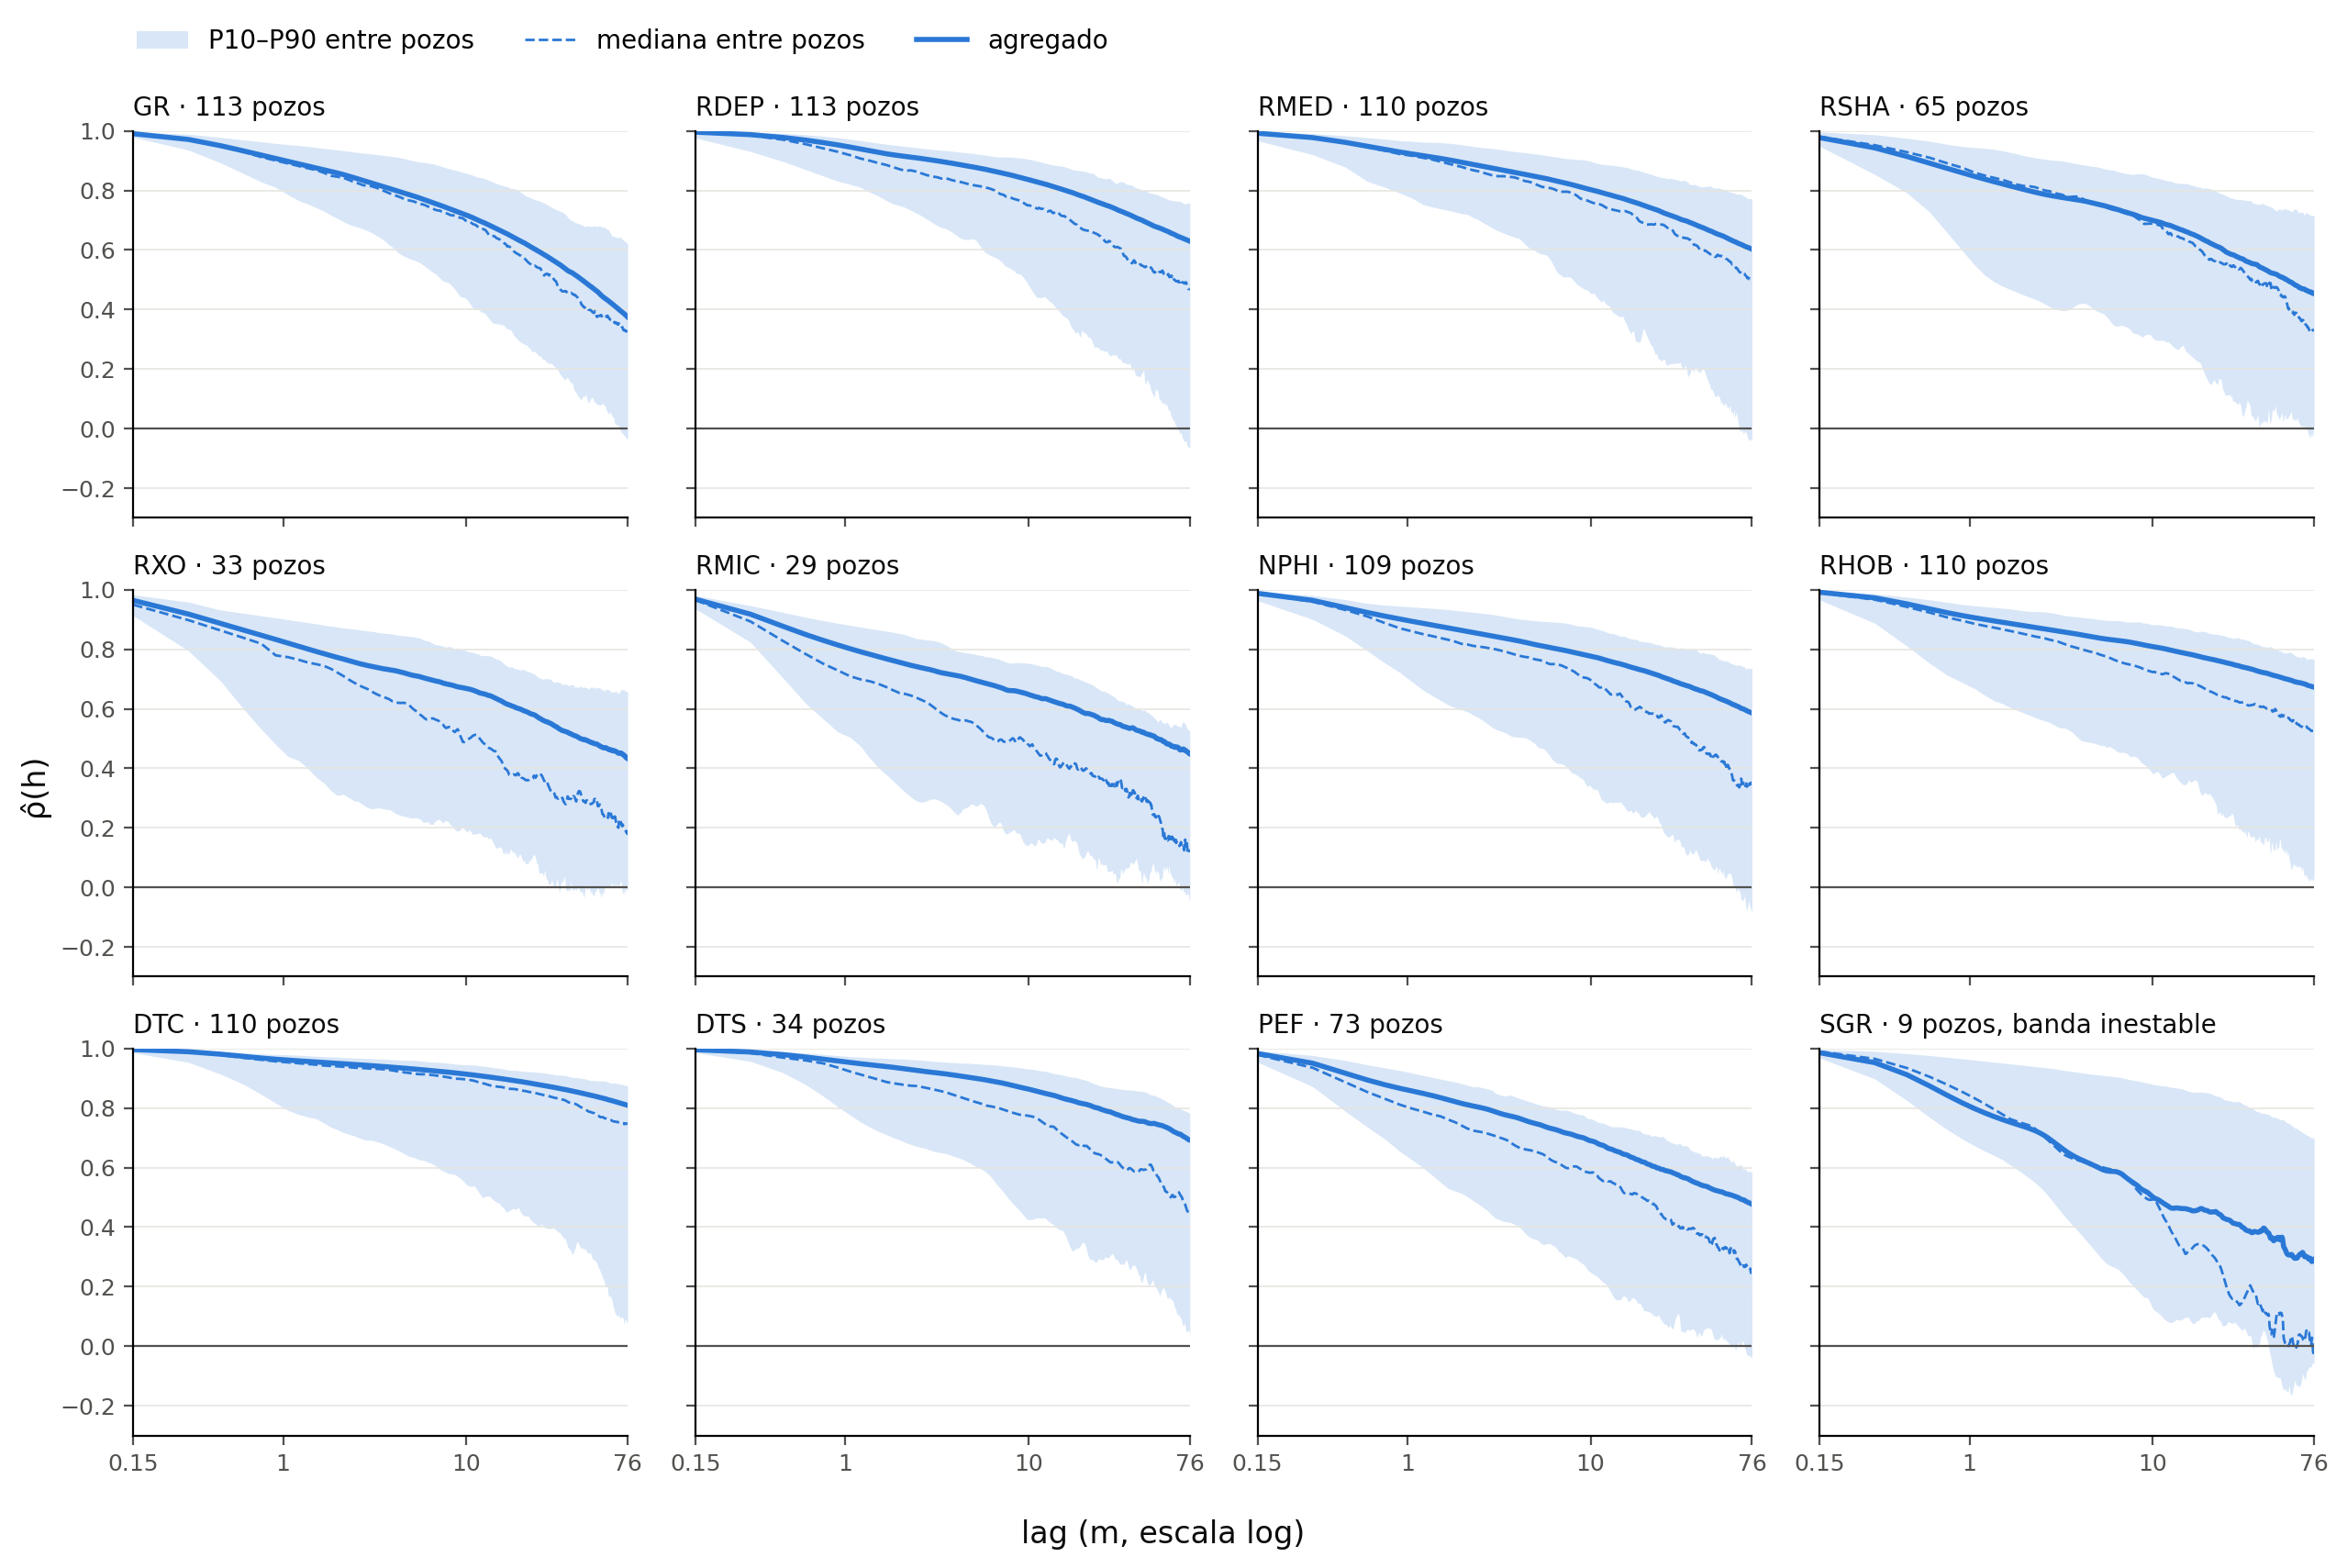
\includegraphics[width=\textwidth]{figuras/etapa3_acf_formacion.png}
\caption{Función de autocorrelación agregada de las 12 curvas que describen la roca, en función de la distancia entre lecturas (escala logarítmica). La línea continua es la autocorrelación agregada sobre los tramos de al menos 2\,000 posiciones, la discontinua es la mediana entre pozos y la banda contiene el 80\,\% central de los pozos. Las resistividades y el factor fotoeléctrico están en escala logarítmica.}
\label{fig:acf}
\end{figure}

\paragraph{Autocorrelación parcial.} Parte del parecido entre dos lecturas lejanas no es directo, sino que se transmite en cadena a través de las lecturas intermedias. La autocorrelación parcial a distancia $h$ mide la correlación entre dos lecturas una vez descontado el efecto lineal de todas las que hay entre ellas, y se calculó a partir de la autocorrelación agregada con el algoritmo de Durbin y Levinson del curso. En \texttt{GR} es apreciable en las siete primeras posiciones y desde la octava, a 1.2~m, queda por debajo de 0.025. El vínculo directo de la curva alcanza entonces cerca de un metro, y todo el parecido a mayor distancia se hereda a través de las lecturas intermedias. En las 12 curvas de la roca esta escala directa está entre 0.9 y 1.7~m, la más gruesa en la resistividad profunda. Es plausible que corresponda al volumen de roca que cada herramienta integra en una lectura, aunque no se verificó con las especificaciones de los instrumentos.

\paragraph{Estacionariedad.} Una serie es estacionaria cuando su media no cambia a lo largo de ella y el parecido entre dos puntos depende solo de la distancia que los separa. En la práctica, una serie así puede alejarse de su nivel pero tiende a volver a él, mientras que una caminata aleatoria, en la que cada paso es independiente de dónde se encuentra la serie, puede alejarse sin límite. La prueba de Dickey y Fuller aumentada (ADF) contrasta estas dos posibilidades mediante la regresión
\begin{equation}
\nabla x_t = \alpha + \beta t + \gamma\, x_{t-1} + \sum_{j=1}^{k} \psi_j \nabla x_{t-j} + w_t ,
\end{equation}
donde $\nabla x_t = x_t - x_{t-1}$ es el cambio entre posiciones consecutivas, $\alpha$ y $\beta t$ representan un nivel y una tendencia, los $k$ cambios rezagados absorben la dinámica de corto plazo y $w_t$ es ruido. Si $\gamma = 0$, el cambio no depende del nivel en que estaba la serie y esta se comporta como una caminata aleatoria, que es la hipótesis nula. Si $\gamma < 0$, estar por encima del nivel habitual empuja el siguiente paso hacia abajo, y la serie tiende a volver. Se aplicó una prueba por tramo de al menos 2\,000 posiciones, con el número de rezagos de la configuración usada en el curso y una segunda regla, con más rezagos, como análisis de sensibilidad. En \texttt{GR} la hipótesis de caminata aleatoria se rechaza en la mayoría de los tramos, y en todos los de más de 10\,000 posiciones (Tabla~\ref{tab:adf}). Entre las 12 curvas de la roca el rechazo va del 82\,\% al 99\,\% de los tramos. La curva vuelve a su nivel, pero muy lentamente, porque la mediana del coeficiente estimado $\hat{\gamma}$ es apenas $-0.009$. Por eso la reversión solo se detecta con claridad en tramos largos.

\begin{table}[htbp]
\centering
\small
\caption{Prueba ADF sobre los tramos de \texttt{GR}. Porcentaje de tramos en que se rechaza, al 5\,\%, la hipótesis de caminata aleatoria, según el largo del tramo y la regla usada para elegir el número de rezagos.}
\label{tab:adf}
\begin{tabular}{lrrr}
\toprule
\textbf{Largo del tramo (posiciones)} & \textbf{Tramos} & \textbf{Regla del curso} & \textbf{Regla con más rezagos} \\
\midrule
2\,000 a 5\,000 & 68 & 86.8\,\% & 69.1\,\% \\
5\,000 a 10\,000 & 55 & 90.9\,\% & 87.3\,\% \\
10\,000 o más & 48 & 100\,\% & 100\,\% \\
\midrule
Total & 171 & 91.8\,\% & 83.6\,\% \\
\bottomrule
\end{tabular}
\end{table}

\paragraph{Espectro y memoria larga.} El espectro descompone la variación de una curva según la escala a la que ocurre, de forma parecida a como un análisis granulométrico reparte un sedimento por tamaños de grano. Se estimó promediando los periodogramas de segmentos de 8\,000 posiciones (1.2~km) de todos los pozos. En \texttt{GR}, solo el 8.6\,\% de la varianza está por debajo de 4.6~m, la escala de las capas individuales, mientras que el 67\,\% está por encima de 76~m, la escala de las unidades y formaciones. En las 12 curvas de la roca esas fracciones van del 5\,\% al 32\,\% y del 43\,\% al 72\,\%, respectivamente. La forma del espectro también caracteriza la memoria de la serie. Para un proceso con memoria larga, la potencia $f$ asociada a una longitud de onda $\lambda$ crece aproximadamente como
\begin{equation}
f(\lambda) \propto \lambda^{2d} ,
\end{equation}
de modo que en un gráfico con ambos ejes logarítmicos la pendiente vale $2d$. Un espectro plano ($d = 0$) corresponde a una serie sin memoria, y $d = 1$ a una caminata aleatoria. Entre $0.5$ y $1$ la serie no es estacionaria pero conserva la tendencia a volver a su nivel. El parámetro $d$ se estimó por bandas de escala con la regresión de Geweke y Porter-Hudak que presenta el curso. En las cinco curvas presentes en todos los pozos, $d$ está entre 0.55 y 0.82 en las bandas de 19 a 305~m, lo que reconcilia los resultados anteriores. La autocorrelación cae lentamente porque $d > 0$, la prueba ADF rechaza la caminata aleatoria porque $d < 1$, y la serie no es estacionaria en sentido estricto porque $d > 0.5$. Las estimaciones de $d$ obtenidas a partir de la autocorrelación y la autocorrelación parcial resultaron sesgadas hacia abajo, y una simulación confirmó que esas fórmulas solo son válidas para $d < 0.5$. Por eso se usó el espectro.

\begin{figure}[htbp]
\centering
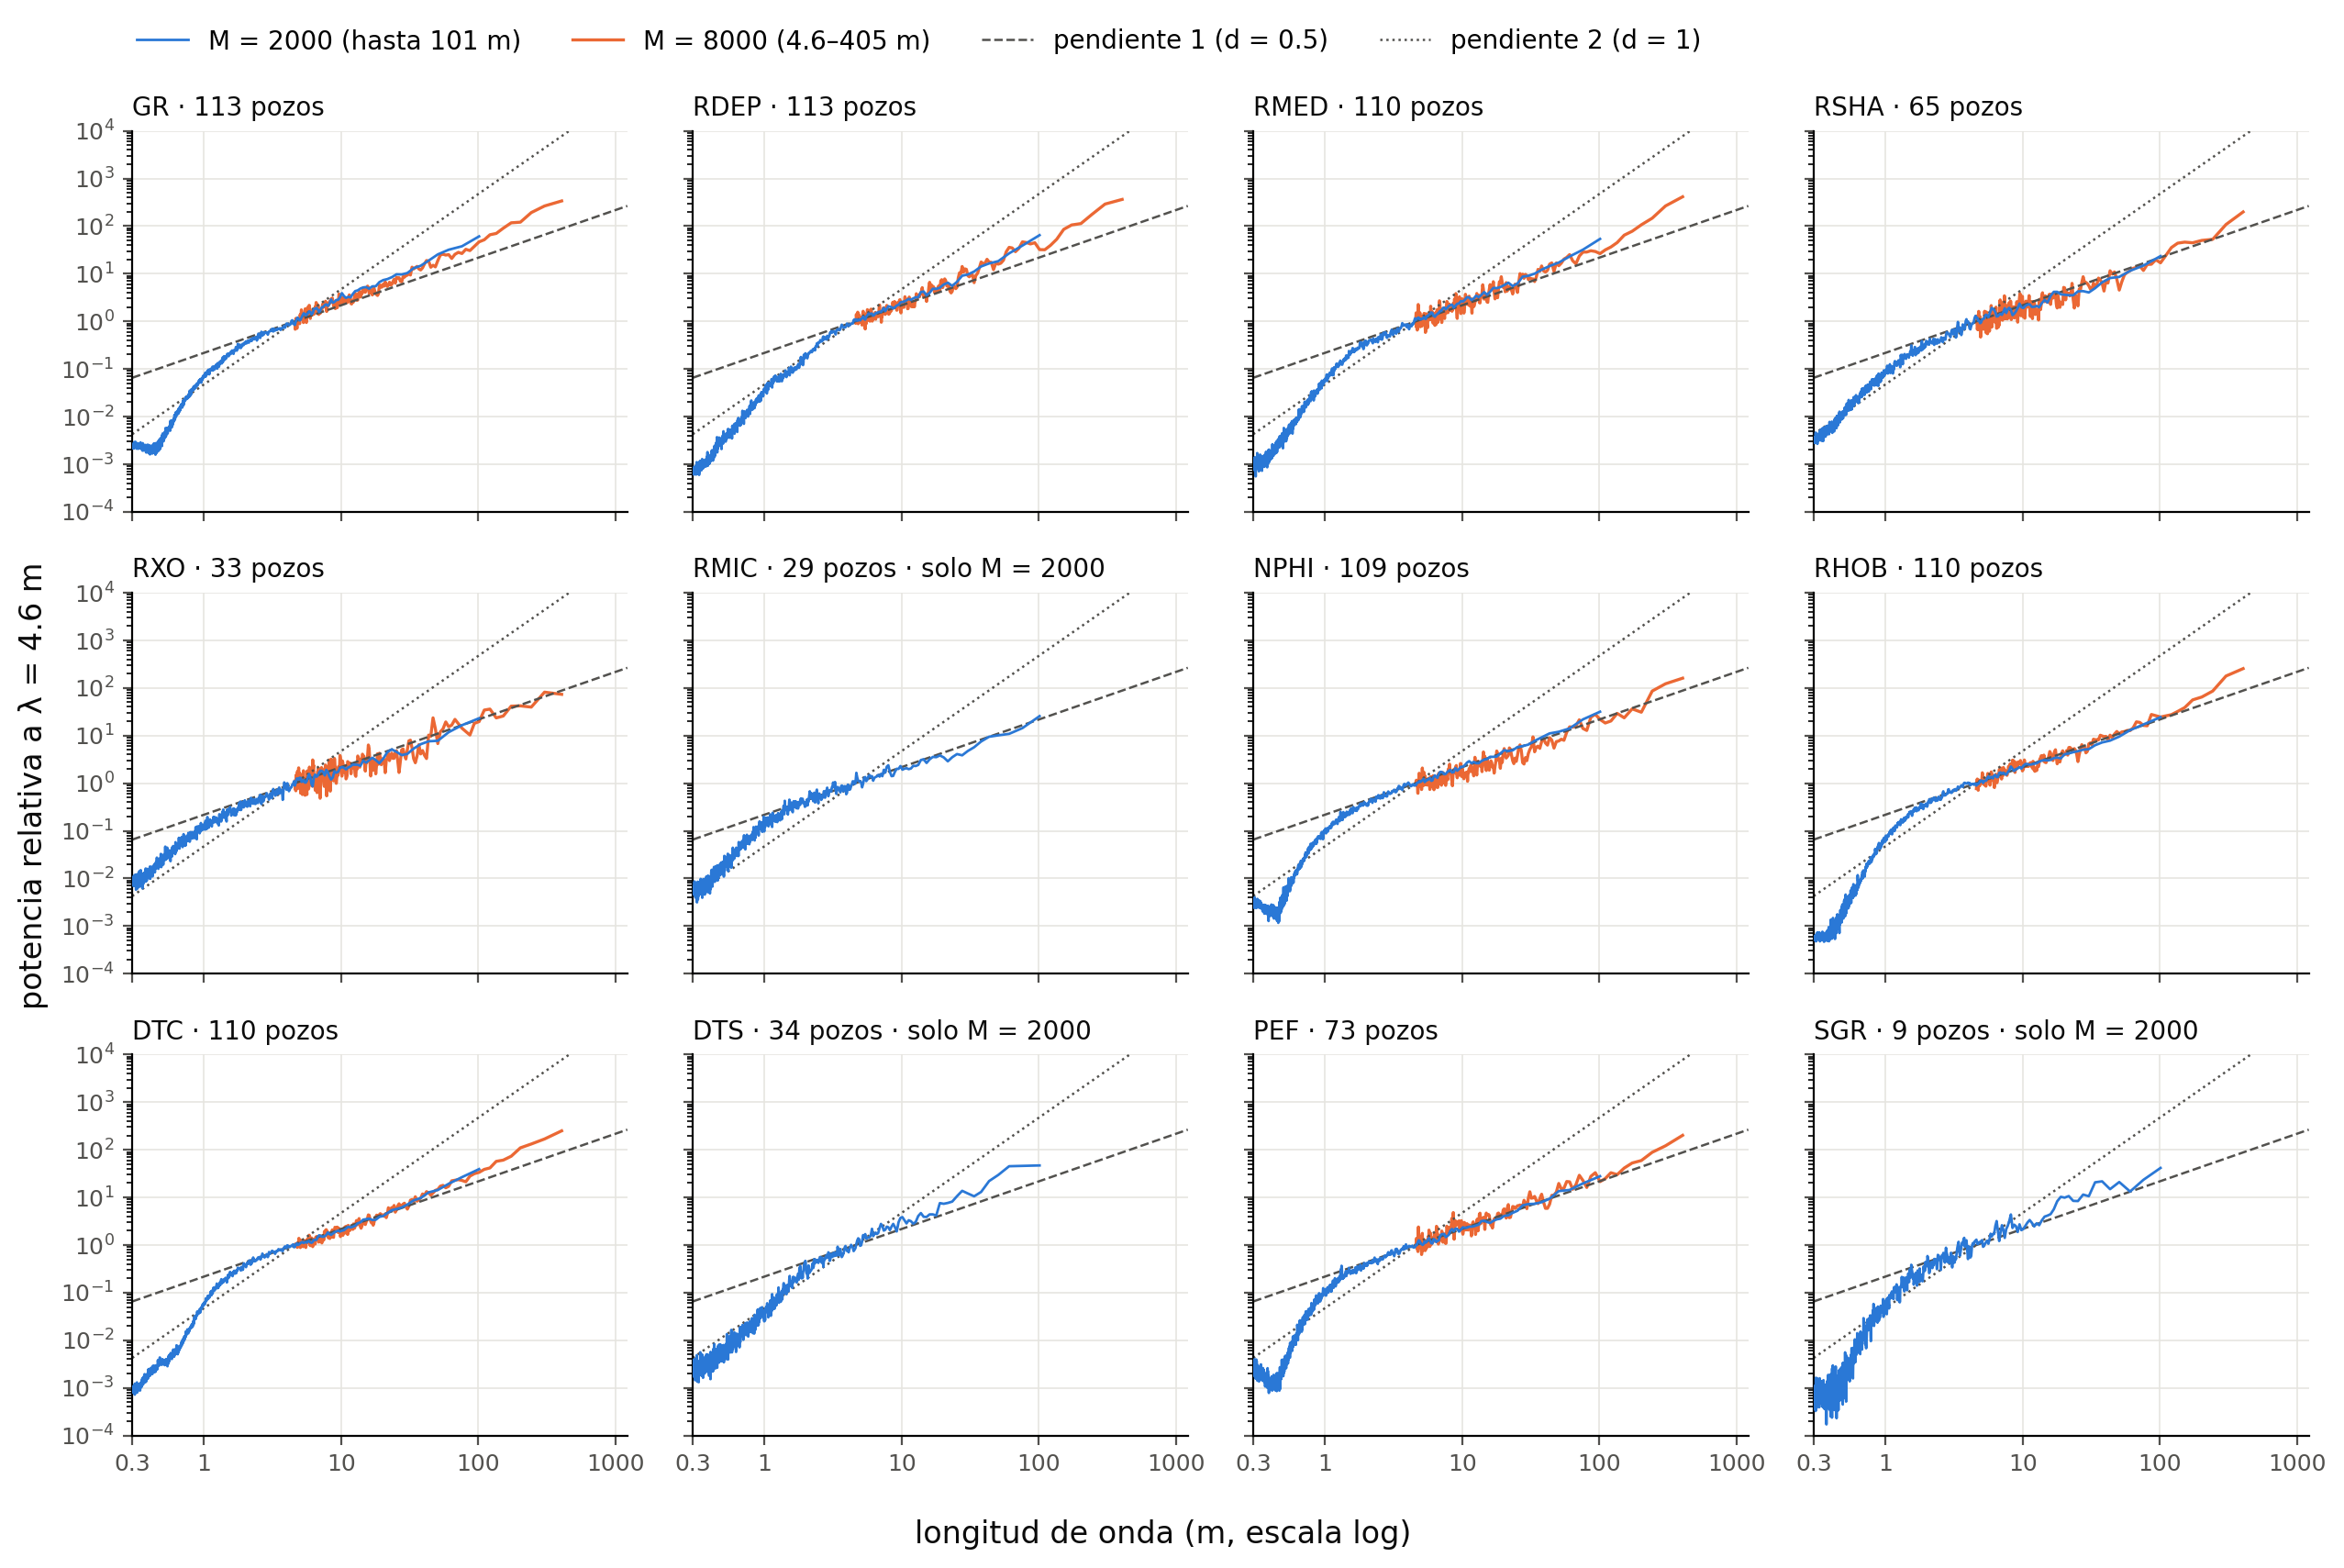
\includegraphics[width=\textwidth]{figuras/etapa3_espectro_formacion.png}
\caption{Espectro agregado de las 12 curvas que describen la roca, normalizado a la potencia en 4.6~m, con ambos ejes en escala logarítmica. En azul, segmentos de 2\,000 posiciones; en naranja, segmentos de 8\,000 posiciones. Las rectas de referencia tienen pendiente 1 ($d = 0.5$) y 2 ($d = 1$). Ninguna curva muestra una meseta entre unos 5 y 100~m.}
\label{fig:espectro}
\end{figure}

El hallazgo más importante para el diseño del modelo está en la Figura~\ref{fig:espectro}. Si existiera una distancia a partir de la cual las lecturas dejan de parecerse, el espectro se aplanaría a partir de esa escala, como la meseta de un variograma. Ninguna de las 12 curvas muestra esa meseta entre unos 5 y 100~m. Entre 200 y 400~m varias incluso se empinan, lo que indica que a escala de formación se comportan como escalones, aunque con confianza moderada porque son las escalas menos promediadas. El único quiebre claro está en el extremo fino. El espectro cae con fuerza por debajo de 1 a 2~m, en coherencia con la escala directa de la autocorrelación parcial.

\paragraph{Curvas que no describen la roca.} Las curvas que reflejan el estado del pozo o la operación de perforación tienen escalas propias. El diámetro del agujero (\texttt{CALI}) es muy persistente por los escalones que imponen los cambios de broca, la corrección de densidad (\texttt{DRHO}) es la menos persistente del conjunto, el potencial espontáneo corregido está dominado por la deriva de su nivel de referencia y la prueba ADF lo rechaza solo en el 52.5\,\% de los tramos, y el peso del lodo se comporta como una función escalonada que describe el programa de perforación y no la roca. Por esta razón, estas curvas no intervinieron en la elección de la ventana de contexto.

\paragraph{Síntesis.} Las curvas que describen la roca tienen dos escalas bien definidas y un comportamiento sin escala entre ellas. En el extremo fino, su resolución directa es de aproximadamente 1~m. En el extremo grueso, la mayor parte de su variación ocurre a escala de formación. Entre ambos extremos la variación crece de forma continua con la escala, de modo que no existe una distancia de independencia que pueda leerse en los datos. Esto tiene dos consecuencias para el diseño. La primera es que el tamaño de la ventana de contexto no puede fijarse como la distancia a la que se pierde la correlación, porque esa distancia no existe, y requiere un criterio explícito distinto basado en los cambios de roca que muestran las curvas, que se desarrolla en la sección~\ref{sec:eda-patrones} y conduce a una ventana de 339 posiciones (51.5~m). La segunda es que la escala directa de aproximadamente 1~m es la referencia física para la distancia máxima a la que se interpolan los huecos interiores, fijada en 8 posiciones (1.2~m) en esa misma sección.

\subsubsection{Identificación de patrones relevantes}
\label{sec:eda-patrones}

La sección anterior describió cada curva por separado. Esta se ocupa de dos preguntas que dependen de mirar varias curvas a la vez. La primera es cómo se relacionan entre sí y a qué escala comparten información. La segunda es dónde cambia la roca a lo largo del pozo y qué tan gruesas son las capas que esos cambios delimitan. De las respuestas salen los dos parámetros de diseño que la Sección~\ref{sec:eda-descriptivo} dejó anunciados, el tamaño de la ventana $W$ y la longitud máxima de hueco que se puede rellenar. Ninguno de los análisis de esta sección usa la etiqueta de litofacies.

\paragraph{Relación entre curvas.} Para medir cuánto se parecen dos curvas a lo largo del pozo se usó la correlación cruzada, que generaliza la autocorrelación a un par de series \cite{shumway2011}. Calculada sobre las curvas tal como se registraron, las correlaciones son altas. La porosidad neutrón y la lentitud del sonido alcanzan 0.79, y la densidad y la lentitud del sonido $-0.80$. Ese valor, sin embargo, mezcla dos cosas. Cada curva es muy persistente y tiende a subir o bajar junto con las demás cuando el pozo pasa de una formación a otra. Una parte grande de la correlación refleja ese cambio lento compartido y no la respuesta de las curvas a cada capa. Para separar ambos efectos se aplicó el preblanqueo del libro guía \cite[Ej.~5.7]{shumway2011}. Se ajustó a la primera curva de cada par un modelo autorregresivo, que describe cuánto de cada lectura se predice con las anteriores, y se aplicó el mismo filtro a las dos curvas. Lo que queda son las variaciones nuevas de cada posición, y su correlación mide la relación a escala de capa. La Tabla~\ref{tab:relacion-curvas} muestra el efecto. Después del preblanqueo las correlaciones entre las cinco curvas núcleo bajan a valores entre 0.02 y 0.14 en valor absoluto. El par de las dos resistividades (\texttt{RDEP} y \texttt{RMED}), que miden casi lo mismo a distinta profundidad de lectura, se incluye como control y conserva 0.61.

La correlación cruzada también sirve para comprobar que las curvas están bien alineadas en profundidad. Si una herramienta registrara los eventos unos centímetros más abajo que otra, el máximo de la correlación aparecería corrido. En 10 de los 12 pares analizados (los once de la Tabla~\ref{tab:relacion-curvas} y el par \texttt{PEF}/\texttt{RHOB}) el máximo está en la misma posición, y en los pares con señal suficiente entre el 79\,\% y el 86\,\% de los pozos tiene su máximo a una posición o menos de distancia. El desfase típico entre curvas es menor de 0.3\,m. Se encontraron dos excepciones puntuales, un desfase de unos 0.6\,m entre \texttt{PEF} y \texttt{RHOB} en el pozo 25/3-1 y otro de 0.3 a 0.45\,m entre las dos resistividades en seis pozos. La revisión visual de esos pozos no confirmó que el desfase fuera constante a lo largo del pozo, de modo que no se corrigieron y quedaron documentados.

La coherencia completa el cuadro. Es el equivalente de una correlación al cuadrado, pero calculada por separado para cada escala de variación \cite[Sec.~4.6]{shumway2011}. Toma valores entre 0 (ninguna relación lineal a esa escala) y 1 (relación lineal perfecta). Por debajo de 1.2\,m la coherencia entre las curvas núcleo es prácticamente nula (0.002 a 0.007), por debajo del umbral de significancia (0.012 a 0.022 según el par). A esa escala cada herramienta registra su propio ruido y no hay información geológica compartida. Entre 1.2 y 4.6\,m, que es la escala de las capas individuales, la relación existe pero es débil, con un máximo de 0.17 entre densidad y lentitud del sonido. La coherencia crece con la escala y llega a 0.40 entre 19 y 101\,m. Las curvas coinciden más en las unidades gruesas que en las capas delgadas. Esto no significa que aporten poca información para clasificar, porque la coherencia solo mide relaciones lineales y la relación entre curvas puede cambiar con el tipo de roca. Sí indica que a escala de capa las curvas son complementarias y no redundantes. Conviene leer estas relaciones como lo que son. Ninguna curva causa a otra. Todas responden a la misma roca, y por eso se mueven juntas cuando la roca cambia.

\begin{table}[htbp]
\centering
\small
\caption{Relación entre pares de curvas. Correlación en la misma profundidad antes y después del preblanqueo, y coherencia a escala de capa y a escala de unidad gruesa.}
\label{tab:relacion-curvas}
\begin{tabular}{lcccc}
\toprule
 & \multicolumn{2}{c}{\textbf{Correlación}} & \multicolumn{2}{c}{\textbf{Coherencia}} \\
\cmidrule(lr){2-3}\cmidrule(lr){4-5}
\textbf{Par} & \textbf{Cruda} & \textbf{Preblanqueada} & \textbf{1.2 a 4.6\,m} & \textbf{19 a 101\,m} \\
\midrule
\texttt{GR}/\texttt{RDEP}   & $-0.021$ & $-0.036$ & 0.022 & 0.004 \\
\texttt{GR}/\texttt{NPHI}   & $0.371$  & $0.075$  & 0.050 & 0.304 \\
\texttt{GR}/\texttt{RHOB}   & $0.066$  & $-0.017$ & 0.004 & 0.002 \\
\texttt{GR}/\texttt{DTC}    & $0.166$  & $0.062$  & 0.034 & 0.122 \\
\texttt{RDEP}/\texttt{NPHI} & $-0.492$ & $-0.045$ & 0.049 & 0.063 \\
\texttt{RDEP}/\texttt{RHOB} & $0.429$  & $0.074$  & 0.051 & 0.047 \\
\texttt{RDEP}/\texttt{DTC}  & $-0.541$ & $-0.060$ & 0.070 & 0.116 \\
\texttt{NPHI}/\texttt{RHOB} & $-0.595$ & $-0.138$ & 0.101 & 0.143 \\
\texttt{NPHI}/\texttt{DTC}  & $0.794$  & $0.130$  & 0.120 & 0.395 \\
\texttt{RHOB}/\texttt{DTC}  & $-0.795$ & $-0.120$ & 0.165 & 0.234 \\
\midrule
\texttt{RDEP}/\texttt{RMED} (control) & $0.942$ & $0.611$ & 0.618 & 0.893 \\
\bottomrule
\end{tabular}
\end{table}

\paragraph{Dónde cambia la roca.} Un contacto entre dos capas se manifiesta en los registros como un escalón, un cambio más o menos brusco en el nivel de varias curvas a la vez. Para localizar esos escalones de forma automática se usó un método de detección de puntos de cambio llamado PELT \cite{killick2012}. Este método no forma parte del material del curso y se tomó de la literatura estadística. La idea es dividir cada tramo del pozo en segmentos dentro de los cuales las cinco curvas núcleo tienen un nivel aproximadamente constante. El algoritmo busca las posiciones de corte $\tau_1, \dots, \tau_m$ que minimizan
\begin{equation}
\sum_{j=0}^{m} \; \sum_{t=\tau_j+1}^{\tau_{j+1}} \lVert \mathbf{x}_t - \bar{\mathbf{x}}_j \rVert^2 \; + \; \beta\, m ,
\label{eq:pelt}
\end{equation}
donde $\mathbf{x}_t$ reúne los valores de las cinco curvas en la posición $t$ (escaladas dentro de cada pozo para que pesen lo mismo), $\bar{\mathbf{x}}_j$ es su promedio en el segmento $j$ y $\tau_0$ y $\tau_{m+1}$ son el inicio y el fin del tramo. El primer término mide cuánto se alejan las lecturas del nivel de su segmento y baja cada vez que se agrega un corte. El segundo cobra una penalización $\beta$ por cada corte. Un corte solo se acepta si reduce el desajuste en más de lo que cuesta. Con $\beta$ pequeño el algoritmo marca muchos contactos y capas delgadas, y con $\beta$ grande solo los cambios mayores. Es lo mismo que pedirle a un geólogo que describa un pozo con más o menos detalle.

El análisis se hizo sobre los tramos de al menos 2\,000 filas con las cinco curvas presentes (150 tramos de 103 pozos, 782\,355 filas). El segmento mínimo se fijó en 8 filas (1.2\,m), la escala por debajo de la cual las curvas no comparten información. En lugar de elegir un solo valor de $\beta$, se recorrió una grilla de 13 valores entre $10^{0.5}$ y $10^{3.5}$, fijada antes de ver resultados. Cada valor de $\beta$ produce una segmentación, y la Figura~\ref{fig:puntos-cambio} (izquierda) muestra cómo cambia el espesor de los segmentos. En el rango en que la medida es confiable ($\beta$ entre 32 y 562), el espesor mediano pasa de 6.2 a 62\,m y el número de contactos baja de 70 a 8 por kilómetro. La curva no muestra ninguna meseta. Si las rocas de estos pozos tuvieran un espesor de capa típico, habría un rango de $\beta$ en que el número de contactos casi no cambiara, y ese rango no existe. La estratificación es jerárquica, con capas dentro de paquetes y paquetes dentro de formaciones, lo que concuerda con el espectro sin una escala dominante de la Sección~\ref{sec:eda-descriptivo}. Los contactos de un nivel grueso suelen reaparecer en los niveles más finos, aunque no siempre en la misma posición, de modo que la jerarquía es aproximada y no estricta.

\begin{figure}[htbp]
\centering
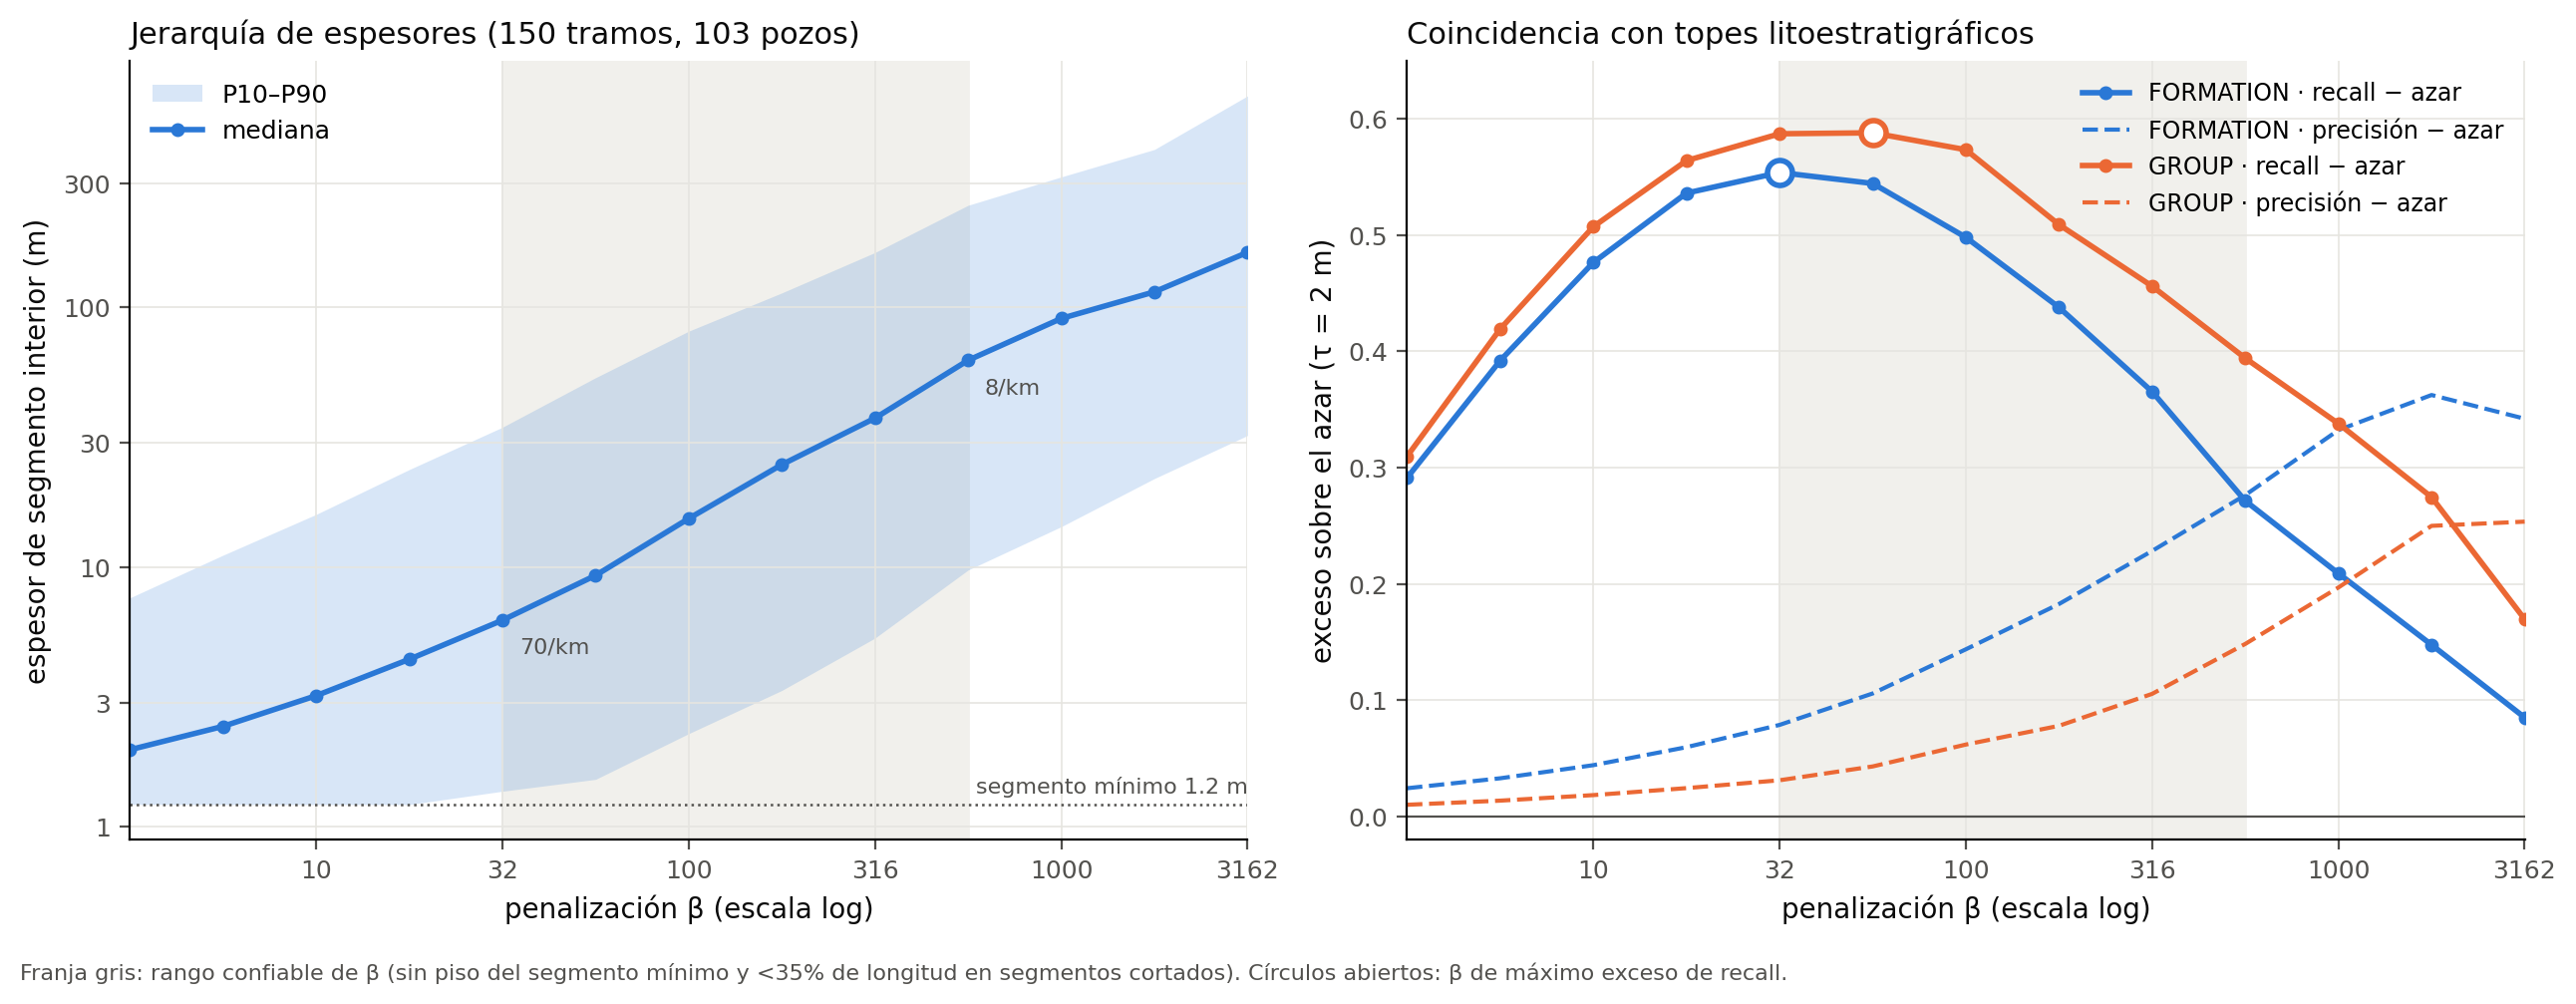
\includegraphics[width=\textwidth]{figuras/etapa3_puntos_cambio.png}
\caption{Puntos de cambio conjuntos de las cinco curvas núcleo. Izquierda, espesor de los segmentos entre contactos (mediana y rango entre los percentiles 10 y 90) en función de la penalización $\beta$, en escala logarítmica. La franja gris marca el rango confiable. No aparece un espesor de capa preferido. Derecha, cuánto superan al azar los contactos detectados al compararlos con los topes de formación y de grupo interpretados en el conjunto de datos, con una tolerancia de 2\,m.}
\label{fig:puntos-cambio}
\end{figure}

Falta saber si esos escalones corresponden a contactos geológicos o a ruido de las herramientas. Para comprobarlo sin usar la etiqueta se recurrió a los topes de formación y de grupo que el conjunto de datos trae interpretados (columnas \texttt{FORMATION} y \texttt{GROUP}). Son límites litoestratigráficos definidos por geólogos, distintos de la litofacies que el modelo debe predecir, y aquí solo sirven como control externo. Para cada $\beta$ se calculó la fracción de topes con un contacto detectado a 2\,m o menos (sensibilidad) y la fracción de contactos detectados con un tope a esa distancia (precisión), y ambas se compararon con lo que se obtendría poniendo el mismo número de cortes al azar. Con $\beta = 31.6$, el 79\,\% de los topes de formación tiene un contacto cercano, frente al 24\,\% que se lograría al azar. En todo el rango de $\beta$ la sensibilidad y la precisión superan al azar entre 3 y 11 veces (Figura~\ref{fig:puntos-cambio}, derecha). Los contactos detectados son, entonces, contactos reales. La mayor ventaja sobre el azar se obtiene con $\beta$ entre 31.6 y 56.2, es decir, cuando los segmentos tienen un espesor mediano de 6 a 9\,m. Esa es la escala a la que la segmentación de las curvas recupera mejor los límites que interpreta un geólogo, y es la que se usa como referencia en lo que sigue.

\paragraph{Tamaño de la ventana.} El modelo clasificará cada muestra mirando una ventana centrada en ella, con $h$ filas por encima y $h$ por debajo, de modo que $W = 2h + 1$ (Sección~\ref{sec:definicion-problema}). Como no existe un espesor de capa único, $W$ no puede leerse directamente de los datos y hay que elegirlo con un criterio explícito. El criterio adoptado es que la ventana centrada en una muestra contenga al menos un contacto en el 90\,\% de las muestras. Una ventana que no alcanza ningún contacto solo ve el interior de una capa homogénea y aporta poco contexto. Una que siempre ve muchos contactos crece sin necesidad. Para aplicarlo se calculó, para cada muestra $i$, la distancia $d_i$ al contacto más cercano, usando los contactos detectados con $\beta = 31.6$,
\begin{equation}
d_i = \min\bigl(d_i^{\uparrow},\, d_i^{\downarrow}\bigr),
\label{eq:distancia-contacto}
\end{equation}
donde $d_i^{\uparrow}$ y $d_i^{\downarrow}$ son las distancias en filas al contacto de arriba y al de abajo. Una ventana de medio ancho $h$ contiene un contacto exactamente cuando $h \ge d_i$, así que basta tomar $h$ igual al percentil 90 de las distancias.

La forma de contar importa. Si se cuentan capas, una capa de 1 fila y otra de 4 pesan lo mismo, la capa típica sale delgada y la ventana resultante ($W = 3$) no ve ningún contacto en las dos muestras del centro de la capa gruesa, es decir, en el 40\,\% de las muestras (Figura~\ref{fig:criterio-w}). Como el modelo centrará una ventana en cada muestra, y las capas gruesas tienen más muestras, el conteo se hizo por muestra, lo que en el ejemplo da $W = 5$. Además, para que los pozos largos no dominen el resultado, cada muestra recibió un peso inverso al número de muestras de su pozo, de modo que todos los pozos pesan lo mismo. Por último, el primer y el último segmento de cada tramo terminan contra el borde del tramo y no contra un contacto, así que su distancia real se desconoce. Se calcularon dos cotas, una que trata el borde como contacto y otra que lo ignora, y se adoptó la segunda por ser la más conservadora. El nivel de 90\,\%, el valor de $\beta$, la ponderación y el tratamiento de los bordes se fijaron antes de ver la distribución de distancias.

\begin{figure}[htbp]
\centering
\begin{tikzpicture}[x=1cm, y=0.7cm, font=\small]
\definecolor{capaA}{HTML}{F6D9C8}
\definecolor{capaB}{HTML}{D4E4F7}
\definecolor{acento}{HTML}{2A78D6}
\definecolor{alerta}{HTML}{EB6834}
\fill[capaA] (0,4) rectangle (2.4,5);
\fill[capaB] (0,0) rectangle (2.4,4);
\foreach \y in {1,2,3} \draw[gray!50] (0,\y) -- (2.4,\y);
\foreach \y in {0,4,5} \draw[very thick] (-0.3,\y) -- (2.7,\y);
\node[left] at (-0.3,5) {contacto};
\node[left] at (-0.3,4) {contacto};
\node[left] at (-0.3,0) {contacto};
\node at (1.2,4.5) {capa delgada};
\node at (1.2,1.5) {capa gruesa};
\node at (3.3,5.6) {$d_i$};
\foreach \y/\d in {4.5/1, 3.5/1, 2.5/2, 1.5/2, 0.5/1} \node at (3.3,\y) {\d};
\fill[alerta] (2.1,2.5) circle (2.5pt);
\draw[alerta, thick] (4.2,1.55) -- (4.4,1.55) -- (4.4,3.45) -- (4.2,3.45);
\node[align=left, anchor=west] at (4.5,2.5) {$W = 3$\\no ve contacto};
\draw[acento, thick] (7.2,0.55) -- (7.4,0.55) -- (7.4,4.45) -- (7.2,4.45);
\node[align=left, anchor=west] at (7.5,2.5) {$W = 5$\\ve el contacto};
\end{tikzpicture}
\caption{Ejemplo del criterio de la ventana con cinco muestras de una fila. La columna $d_i$ indica la distancia de cada muestra al contacto más cercano. Para la muestra marcada ($d_i = 2$), una ventana de 3 filas queda dentro de la capa gruesa y una de 5 filas alcanza el contacto superior.}
\label{fig:criterio-w}
\end{figure}

Con estos criterios, el percentil 90 de las distancias resultó de 24.5 a 25.7\,m según la cota usada en los bordes. Con la cota conservadora se obtiene $h = 169$ filas y una ventana de referencia de $W = 339$ filas, equivalentes a 51.5\,m. La mediana de las distancias es de unos 5\,m, de modo que el tamaño de la ventana lo deciden las muestras que están dentro de capas gruesas. Como contraste, se calcularon con el mismo criterio las ventanas correspondientes a los niveles de detalle vecinos, 231 filas (35.1\,m, $\beta = 17.8$) y 471 filas (71.6\,m, $\beta = 56.2$). Estas dos ventanas solo se evaluarán como análisis de sensibilidad y no reemplazarán a la de referencia, que quedó fijada antes de entrenar cualquier modelo.

El criterio se cumple en promedio, pero no en todos los pozos. Solo el 55\,\% de los pozos alcanza por sí mismo el 90\,\% de muestras con contacto en la ventana, y agrandar la ventana no corrige esa proporción, porque los pozos con menor cobertura tienen capas mucho más gruesas que los demás. Es un rasgo de la geología de esos pozos y no un defecto del criterio. La ventana tiene además un costo pequeño. Hay 54 tramos continuos más cortos que $W$, que suman 5\,683 filas (0.40\,\% del total) en las que no cabe una ventana completa, y otro 5.7\,\% de las filas está tan cerca del borde de su tramo que la ventana centrada se saldría de él. Ningún pozo queda sin ventana. Cómo tratar esas filas se decidirá en la preparación de datos para los modelos.
% Pendiente (Etapa 5): contrastar W con los contactos de litofacies, solo en pozos de entrenamiento. Agregar el resultado cuando exista.
% Pendiente (Etapa 6): \ref al tratamiento de filas sin ventana completa y de borde.

\paragraph{Longitud máxima de interpolación.} La Sección~\ref{sec:eda-limpieza} dejó pendiente cuál es el hueco más largo que se puede rellenar trazando una recta entre los valores vecinos. Se fijó en $G_{\max} = 8$ filas (1.2\,m), que es la resolución vertical de las propias curvas. Tres resultados de este análisis apuntan a esa escala. La escala de dependencia directa de las curvas, estimada con la autocorrelación parcial, va de 0.9 a 1.7\,m. Por debajo de 1.2\,m la coherencia entre curvas es nula. Y solo el 10\,\% de las capas delimitadas con $\beta = 31.6$ mide menos de 1.37\,m. El segmento mínimo de 1.2\,m usado en la detección de contactos es una elección de diseño coherente con esas tres evidencias. Un hueco de ese tamaño no puede esconder un contacto que el análisis sea capaz de resolver.

Para comprobar que interpolar a esa distancia es seguro se hizo un experimento de control. Se ocultaron tramos de $g$ filas con dato real, se rellenaron con una recta y se midió el error dividido por la escala robusta de la curva en el pozo, la misma que se usó en la normalización. Se repitió 3\,000 veces por curva y por largo de hueco, eligiendo primero un pozo al azar y luego una posición. Antes del experimento se fijó una alarma, un error mediano mayor que 0.5 con $g = 8$ en alguna curva de formación. La alarma no se activó. Con $g = 8$ el error mediano va de 0.06 en la resistividad profunda a 0.21 en el factor fotoeléctrico. El error crece de forma continua con el largo del hueco, sin un quiebre en 8 filas, de modo que el experimento confirma la elección pero no habría servido para hacerla. En uno de cada diez huecos el error se acerca a 0.7 en las curvas de lectura más somera (\texttt{RXO}, \texttt{PEF}), por lo que cada valor rellenado irá acompañado de una columna que lo marque como interpolado. Se eligió la interpolación lineal porque no tiene parámetros. Un método ajustado a los datos, como un modelo autorregresivo, usaría información de todos los pozos, incluidos los que más adelante serán de prueba. La recta solo usa los dos vecinos del mismo pozo y del mismo tramo. La regla afecta a 4\,818 celdas, el 2.5\,\% de los faltantes interiores. El 86\,\% de esos faltantes está en huecos de más de 100 filas, que corresponden a intervalos donde la curva no se registró, y seguirá como faltante. La interpolación se aplicará en la preparación de datos para los modelos y no modifica la tabla curada.
% Pendiente (Etapa 6): \ref al pipeline donde se aplica G_max.

\paragraph{Revisión de pozos representativos.} Todo lo anterior se basa en estadísticos agregados de muchos pozos. Para comprobar sobre registros reales que los contactos detectados corresponden a cambios de roca, se examinaron siete pozos elegidos con reglas fijadas antes de graficar. Tres son pozos típicos, uno por cada grupo de pozos según el número de curvas disponibles, elegidos por código como el pozo más cercano al centro de su grupo (34/10-19, 7/1-1 y 16/4-1). Los otros cuatro representan cada uno de los problemas ya documentados, como desfases entre curvas, baja cobertura de la ventana o pérdida de filas por tramos cortos (25/4-5, 31/3-2, 25/3-1 y 34/4-10~R). Las figuras no muestran la litofacies, porque estos pozos pueden quedar en el conjunto de prueba, y la lista no se usará para construir la partición entre entrenamiento y prueba. Las Figuras~\ref{fig:pozo-tipico} y~\ref{fig:pozo-problematico} muestran dos de ellos.

\begin{figure}[p]
\centering
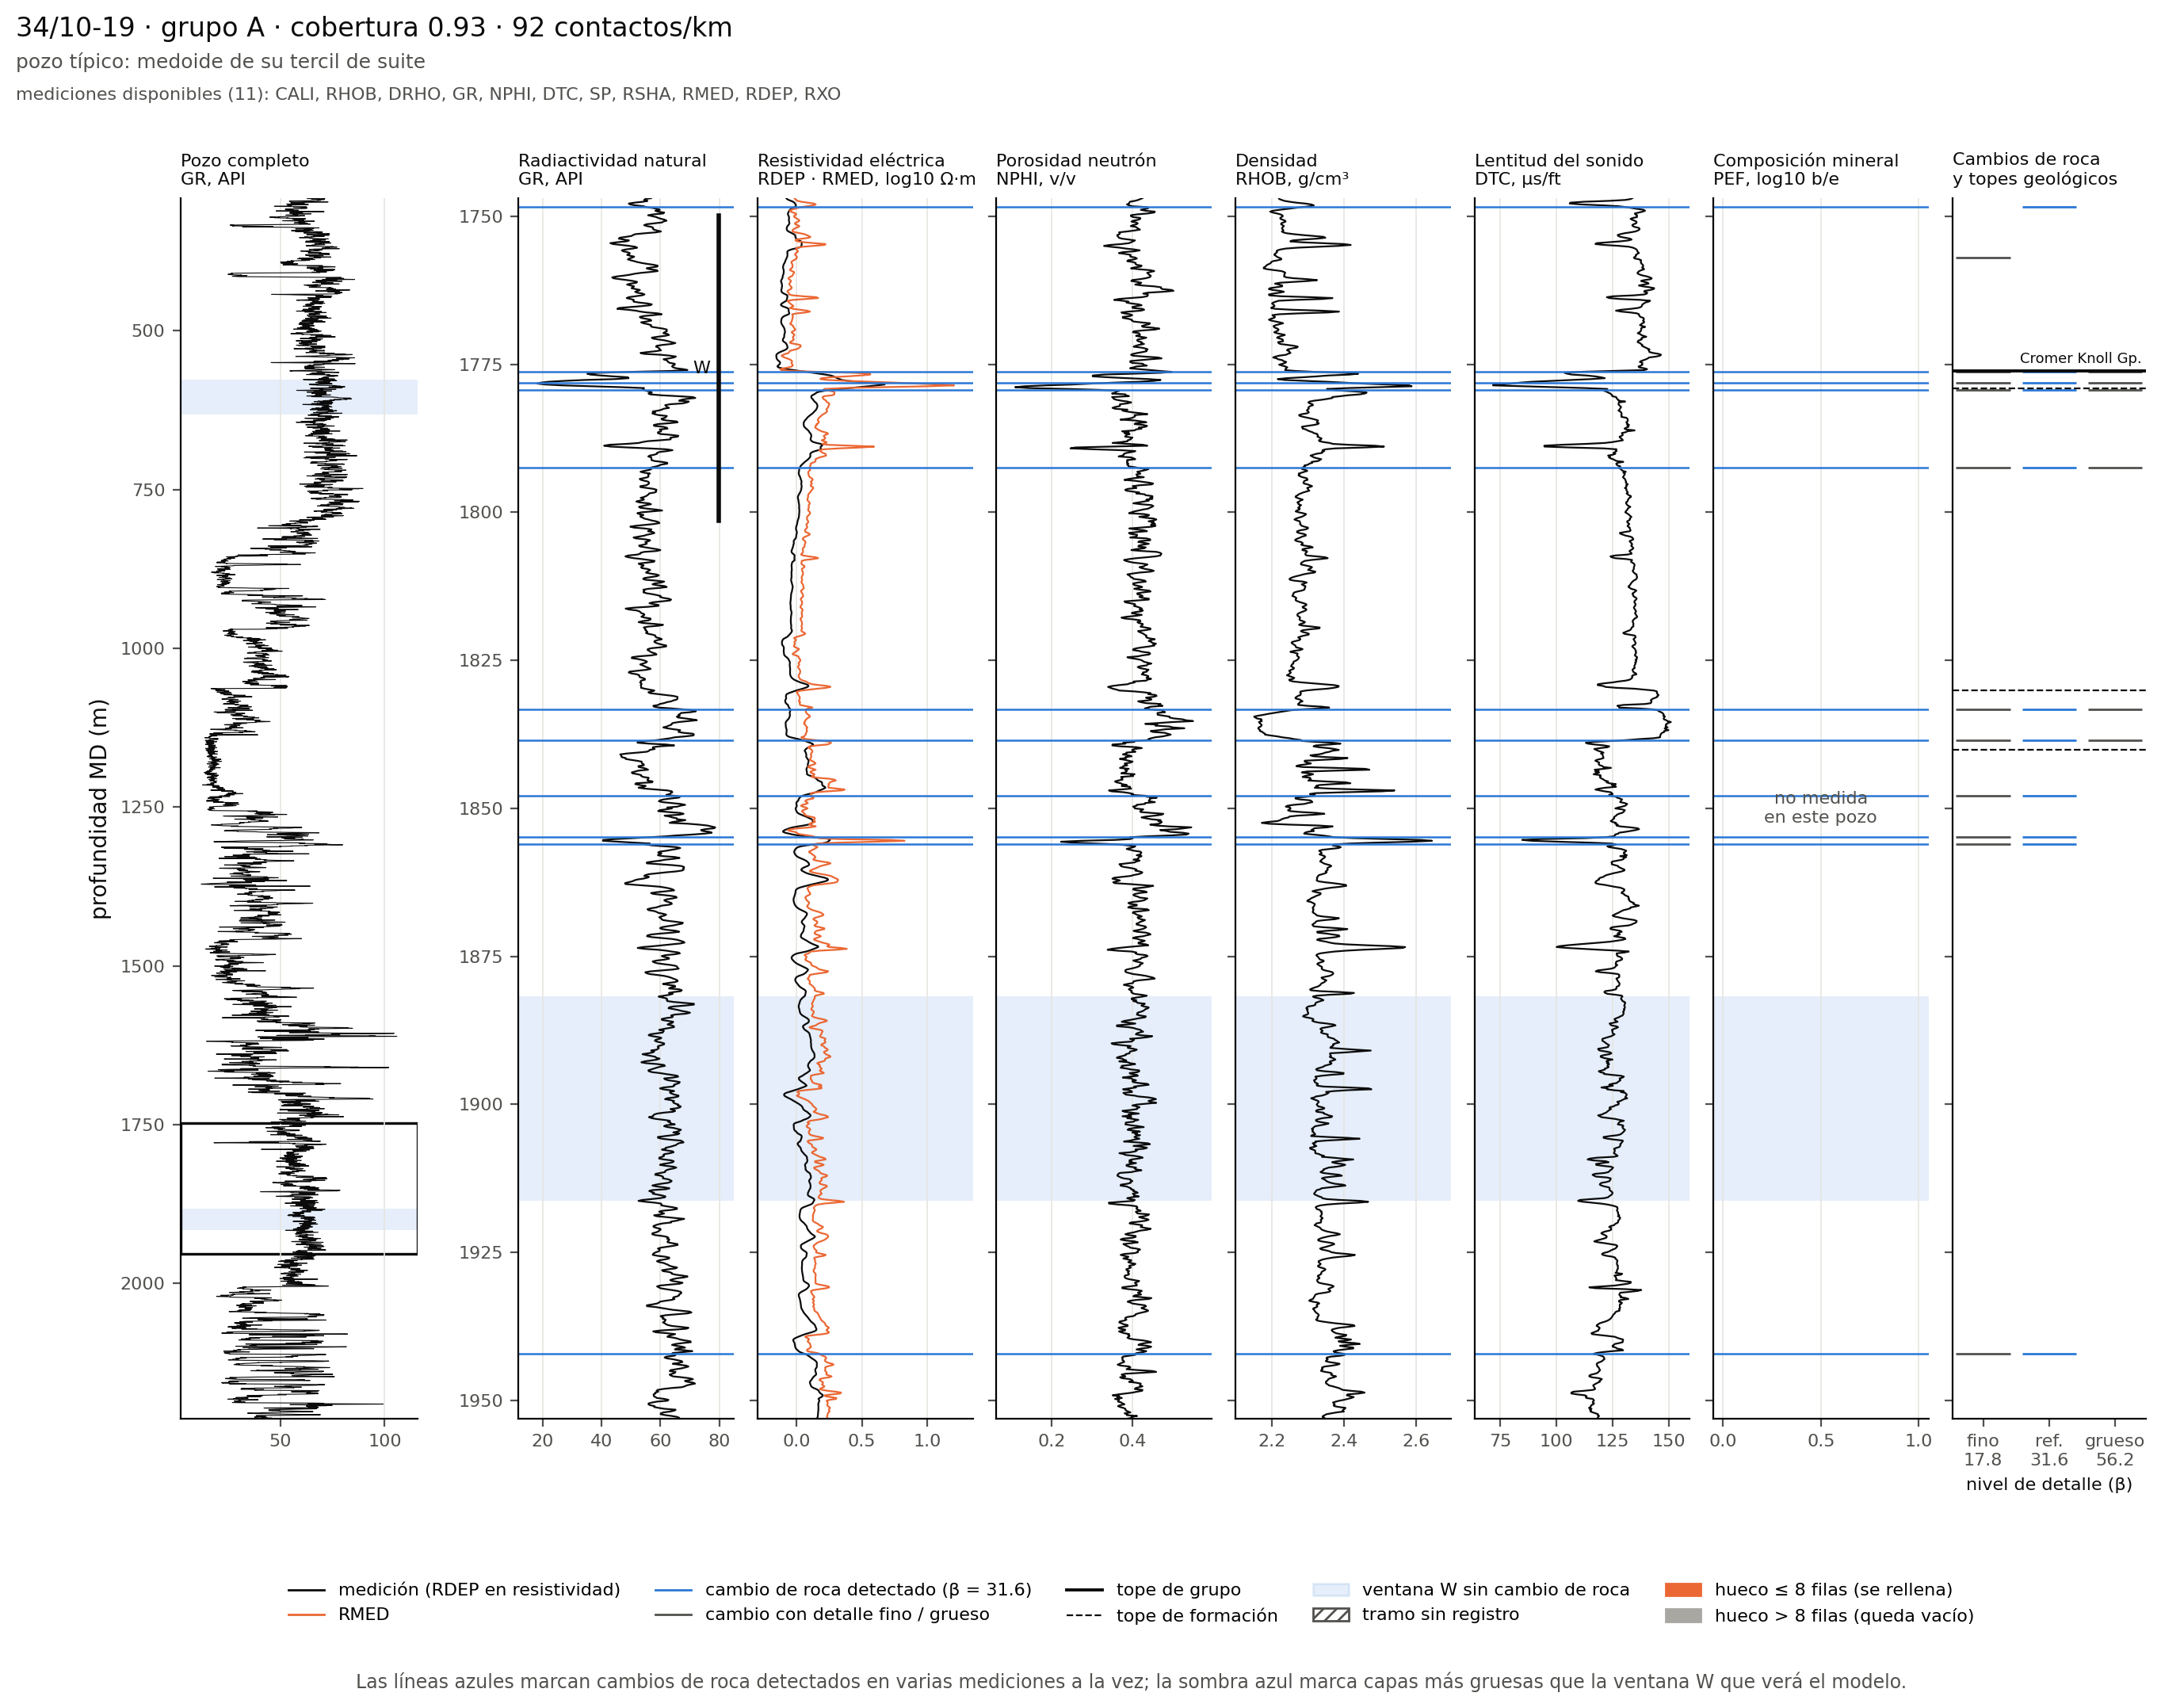
\includegraphics[width=\textwidth]{figuras/etapa3_pozo_34_10-19.png}
\caption{Pozo típico 34/10-19. A la izquierda, la radiactividad natural en todo el pozo, con el intervalo ampliado enmarcado. En las pistas siguientes, seis curvas en ese intervalo de unos 200\,m. Las líneas azules son los contactos detectados con $\beta = 31.6$ y la sombra azul marca las muestras cuya ventana $W$ no contiene ningún contacto. La pista de la derecha compara los contactos a tres niveles de detalle con los topes de grupo y de formación.}
\label{fig:pozo-tipico}
\end{figure}

\begin{figure}[p]
\centering
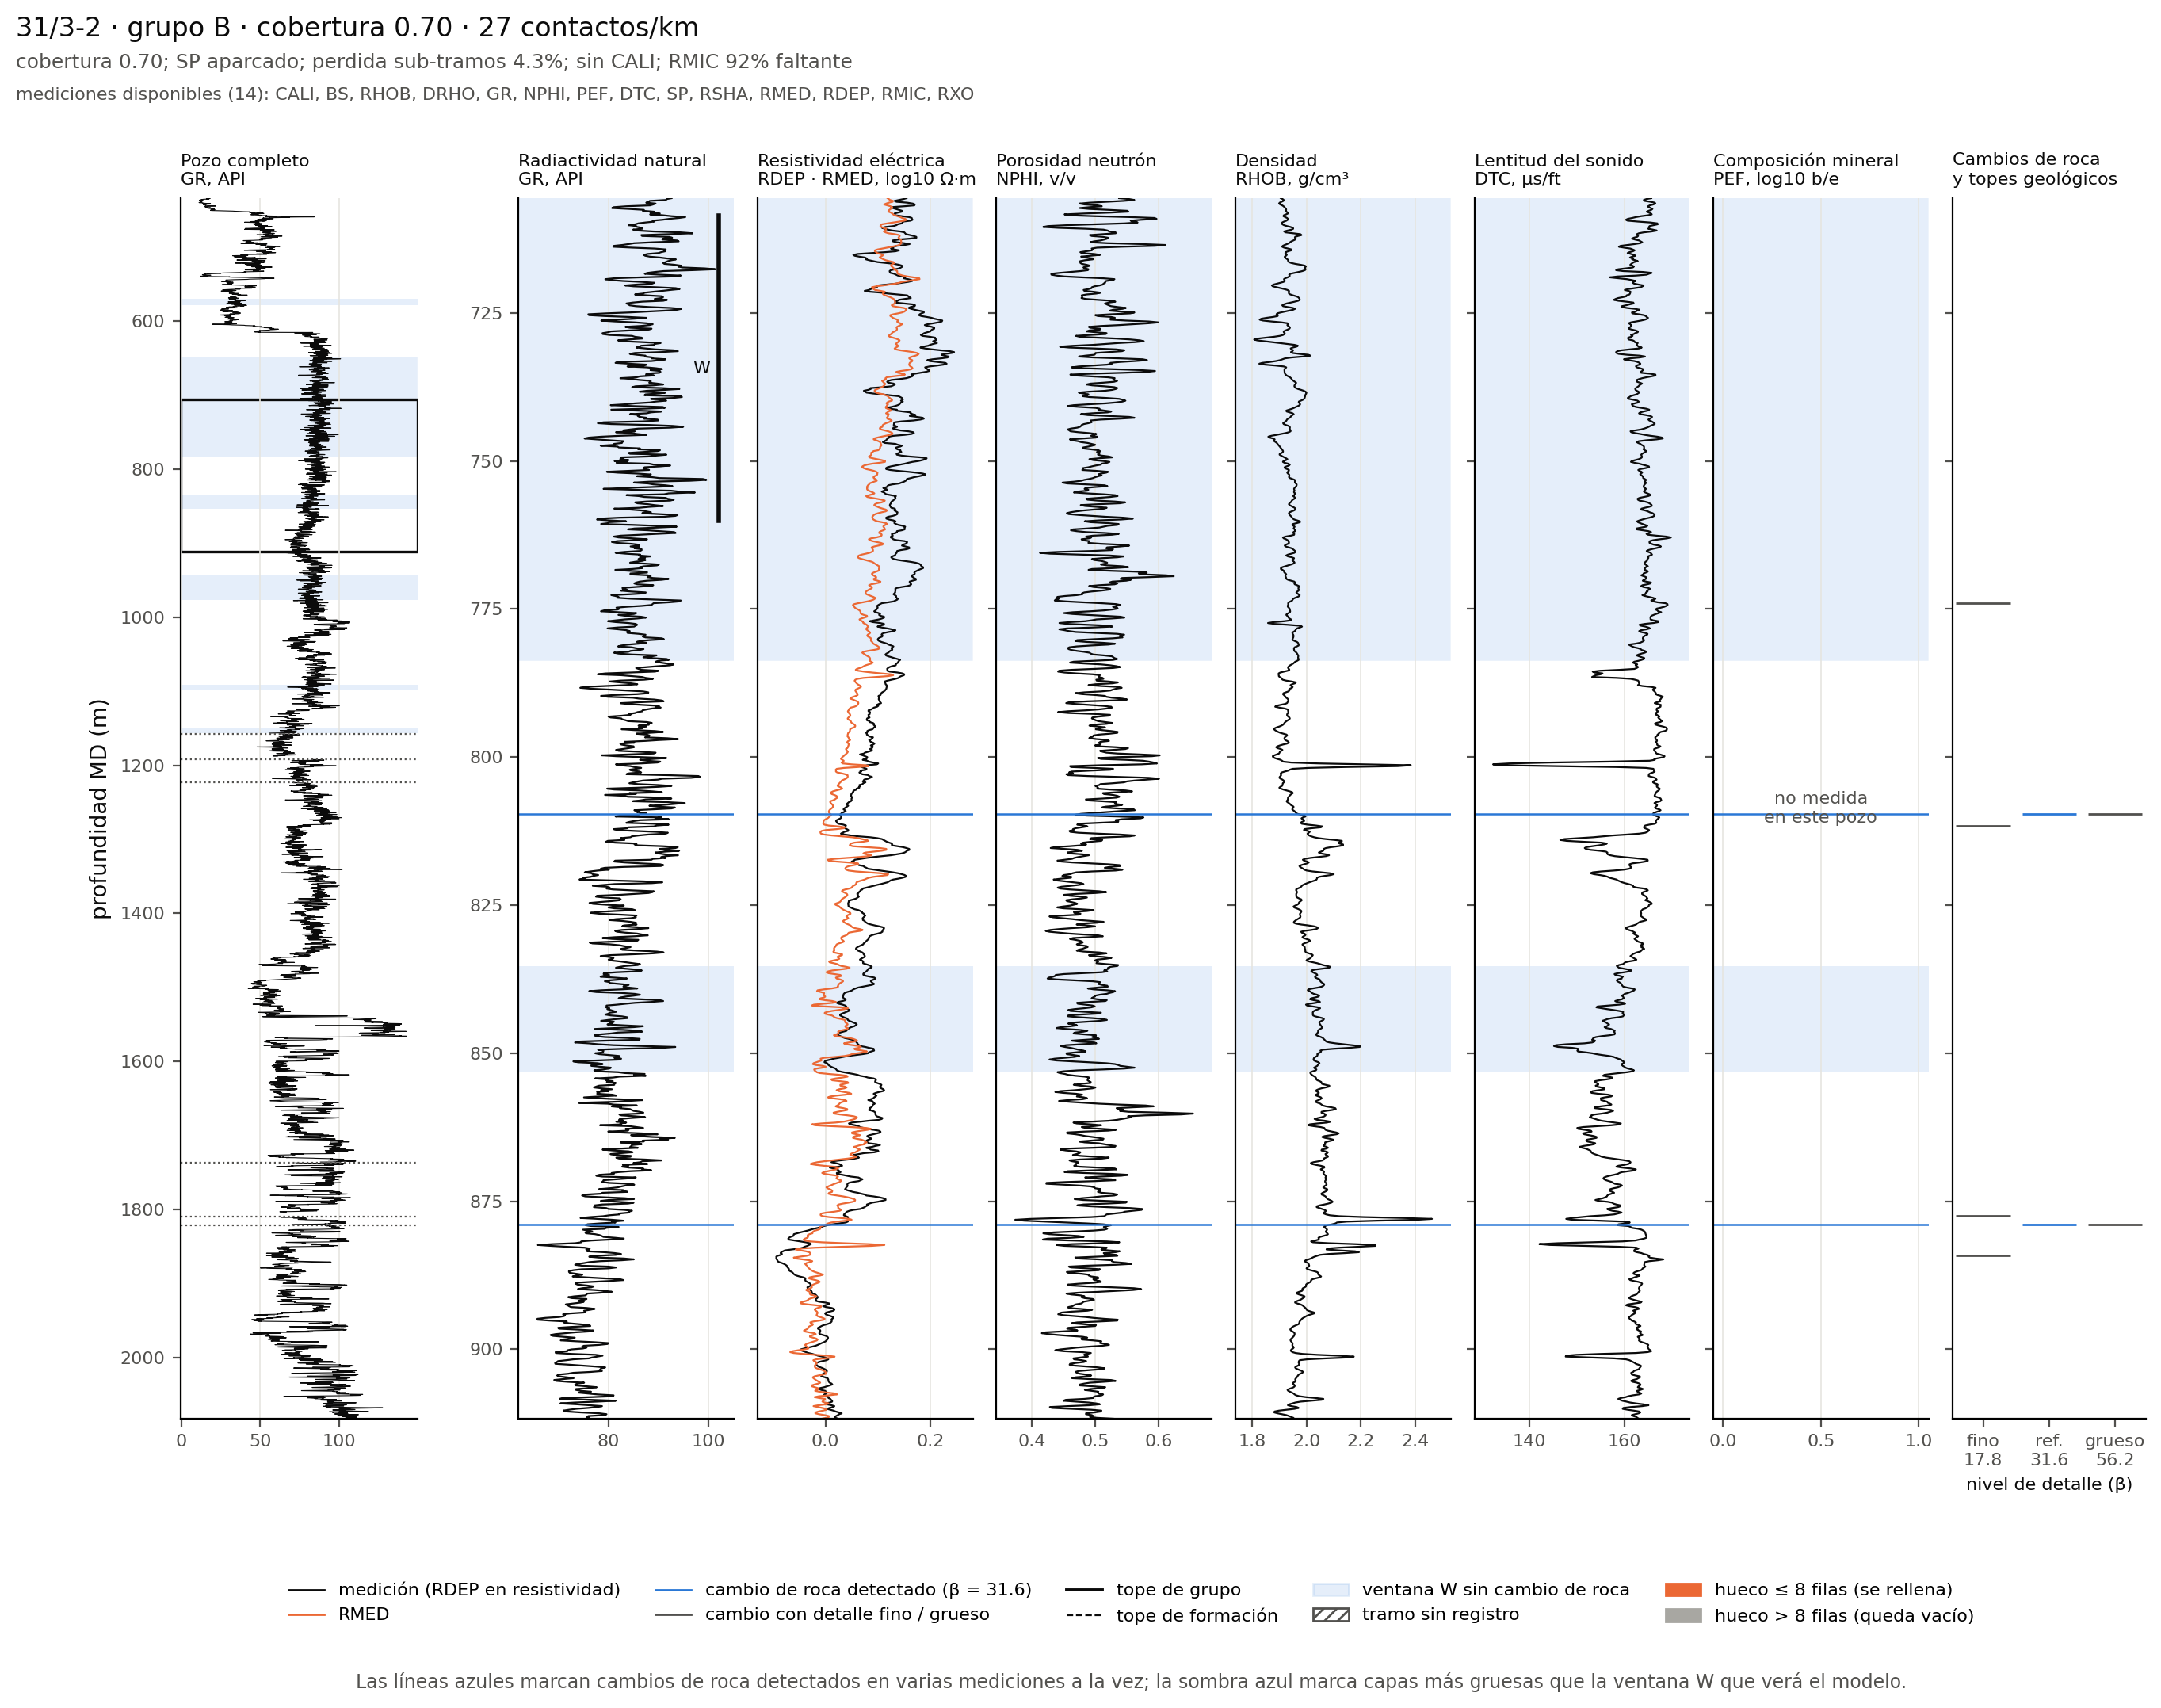
\includegraphics[width=\textwidth]{figuras/etapa3_pozo_31_3-2.png}
\caption{Pozo 31/3-2, el de menor cobertura de la ventana entre los revisados. El intervalo ampliado es una unidad somera de roca blanda y uniforme con solo dos contactos en unos 200\,m. Mismas convenciones que la Figura~\ref{fig:pozo-tipico}.}
\label{fig:pozo-problematico}
\end{figure}

La revisión dejó cuatro observaciones. Primera, los contactos detectados coinciden con escalones simultáneos en varias curvas. En 34/10-19 el contacto de 1\,777\,m, que coincide con el tope del grupo Cromer Knoll, aparece a la vez en la densidad, la porosidad y el sonido, y en ninguno de los pozos se vio un contacto producido por un pico de una sola curva. Segunda, las zonas donde la ventana no alcanza un contacto son unidades gruesas y homogéneas. En 31/3-2, el intervalo ampliado tiene solo dos contactos en unos 200\,m de roca uniforme, lo que explica su baja cobertura. Tercera, las capas de menos de 1.2\,m no generan contacto, como el pico delgado de densidad y sonido a 801\,m en ese mismo pozo. Por esa razón la ventana elegida tiende a ser conservadora. Cuarta, el pozo 34/4-10~R muestra escalones claros pero ningún contacto, porque su tramo continuo más largo con las cinco curvas núcleo (1\,762 filas) no alcanzó el mínimo de 2\,000 filas y quedó fuera de la detección. Es una limitación del alcance del análisis y no de la geología. Ninguna de estas observaciones llevó a modificar $W$, $\beta$ ni $G_{\max}$.

\paragraph{Síntesis.} La Tabla~\ref{tab:escala-vertical} reúne las escalas verticales encontradas en esta sección y en la anterior. La estratificación de estos pozos es jerárquica y no tiene un espesor característico. La resolución de las curvas fija el límite inferior, alrededor de 1.2\,m, y la ventana del modelo, de unos 50\,m, abarca capas de pocos metros a decenas de metros. A esa escala el cambio de formación aparece dentro de la ventana casi como un desplazamiento constante del nivel de las curvas.

\begin{table}[htbp]
\centering
\small
\caption{Escalas verticales encontradas en el análisis exploratorio.}
\label{tab:escala-vertical}
\begin{tabular}{p{5.2cm}p{4.2cm}p{4.8cm}}
\toprule
\textbf{Escala} & \textbf{Valor} & \textbf{Evidencia} \\
\midrule
Resolución propia de las curvas & 0.9 a 1.7\,m & Autocorrelación parcial y espectro \\
Escala mínima con información compartida entre curvas & 1.2\,m & Coherencia nula por debajo \\
Longitud máxima de interpolación ($G_{\max}$) & 1.2\,m (8 filas) & Resolución de las curvas \\
Espesor típico de capa & Sin escala única, mediana de 6 a 62\,m & Puntos de cambio sin meseta y espectro sin escala dominante \\
Escala que mejor recupera los límites geológicos & 6 a 9\,m de espesor mediano & Comparación con topes de formación y de grupo \\
Distancia de una muestra al contacto más cercano & Mediana de 5\,m, percentil 90 de 24.5 a 25.7\,m & Contactos con $\beta = 31.6$ \\
Ventana del modelo ($W$) & 51.5\,m (339 filas) & Contacto en el 90\,\% de las muestras \\
Escala de formación & Más de 76\,m (43 a 72\,\% de la varianza) & Espectro \\
\bottomrule
\end{tabular}
\end{table}

\subsection{Modelado}

\subsubsection{Métodos Estadísticos y Líneas Base}
\begin{itemize}
    \item \textbf{Modelos de referencia:}
    \item \textbf{Supuestos e interpretación:}
\end{itemize}

\subsubsection{Aprendizaje Profundo}
\begin{itemize}
    \item \textbf{Arquitecturas:}
    \item \textbf{Función de pérdida y optimización:}
    \item \textbf{Estrategia de entrenamiento:}
\end{itemize}

\subsubsection{Evaluación}
\begin{itemize}
    \item \textbf{Métricas:}
    \item \textbf{Estrategia de validación:}
    \item \textbf{Comparación de enfoques:}
\end{itemize}

% ==========================================
% 4. TECNOLOGÍA - SISTEMAS DE ML (MLOps)
% ==========================================
\section{Tecnología - Sistemas de Aprendizaje Automático (MLOps)}

\subsection{Datos}

\subsection{Procesamiento}

\subsection{Entrenamiento}

\subsection{Almacenamiento}

\subsection{Despliegue}

\subsection{Aplicación}

% ==========================================
% 5. RESULTADOS
% ==========================================
\section{Resultados}

\subsection{Análisis de desempeño}
\begin{table}[H]
\centering
\caption{Comparativa de desempeño en el conjunto de prueba (pozos no vistos).}
\label{tab:resultados}
\begin{tabular}{lccc}
\toprule
\textbf{Modelo} & \textbf{Accuracy} & \textbf{F1-Score Macro} & \textbf{F1-Score Ponderado} \\
\midrule
Línea Base (Punto a Punto) & -- & -- & -- \\
Bi-LSTM Secuencial & -- & -- & -- \\
Transformer (Atención) & -- & -- & -- \\
\bottomrule
\end{tabular}
\end{table}

\subsection{Interpretación de resultados}

\subsection{Limitaciones}


% ==========================================
% 6. CONCLUSIONES
% ==========================================
\section{Conclusiones}

\subsection{Aportes del proyecto}

\subsection{Posibles mejoras y trabajo futuro}

% ==========================================
% 7. REFERENCIAS BIBLIOGRÁFICAS
% ==========================================
\printbibliography[heading=bibintoc,title={Referencias}]

\end{document}